\documentclass[a4paper]{article}
\renewcommand{\epsilon}{\varepsilon}
\newcommand{\triposcourse}{Methods}
\usepackage{fancyhdr,titlesec,geometry}
\usepackage[dvipsnames]{xcolor}
\usepackage[many]{tcolorbox}
\usepackage{xifthen}
\usepackage{import}
\usepackage{parskip}
\usepackage{transparent}
\usepackage{mathtools,amssymb,amsfonts,amsthm,bm}   % Math Presets
\usepackage{array,tabularx,booktabs}                % Table Presets
\usepackage{graphicx,wrapfig,float,caption}         % Figure Presets
\usepackage{setspace,multicol}                      % Text Presets
\usepackage{tikz,physics,cancel,tkz-euclide,pgfplots,tikz-3dplot}                    % Physics Presets
\usepackage{amsmath}
\usepackage{mathrsfs}
\usepackage{enumerate}
\usepackage[shortlabels]{enumitem}
\usepackage{hyperref}
\usepackage{lipsum}
\usepackage{IEEEtrantools}
\usepackage{xcomment}
\usepackage{sectsty}
\usepackage{thmtools}
\usepackage{mdframed}
\usepackage{siunitx}
\usepackage{centernot}

\newcommand{\sectionbreak}{\clearpage}

\tdplotsetmaincoords{60}{120}

\usetikzlibrary{arrows.meta}
\usetikzlibrary{decorations.markings}
\usetikzlibrary{decorations.pathmorphing}
\usetikzlibrary{automata, positioning}
\usetikzlibrary{fadings}
\usetikzlibrary{intersections}
\usetikzlibrary{cd}
\usetikzlibrary{patterns}
\usetikzlibrary{shapes.arrows}
\usepgfplotslibrary{colormaps, external}
\pgfarrowsdeclarecombine{twolatex'}{twolatex'}{latex'}{latex'}{latex'}{latex'}
\tikzset{->/.style = {decoration={markings,
                                  mark=at position 1 with {\arrow[scale=1.6]{latex'}}},
                      postaction={decorate}}}
\tikzset{<-/.style = {decoration={markings,
                                  mark=at position 0 with {\arrowreversed[scale=1.6]{latex'}}},
                      postaction={decorate}}}
\tikzset{<->/.style = {decoration={markings,
                                   mark=at position 0 with {\arrowreversed[scale=1.6]{latex'}},
                                   mark=at position 1 with {\arrow[scale=1.6]{latex'}}},
                       postaction={decorate}}}
\tikzset{->-/.style = {decoration={markings,
                                   mark=at position #1 with {\arrow[scale=1.6]{latex'}}},
                       postaction={decorate}}}
\tikzset{-<-/.style = {decoration={markings,
                                   mark=at position #1 with {\arrowreversed[scale=1.6]{latex'}}},
                       postaction={decorate}}}
\tikzset{->>/.style = {decoration={markings,
                                  mark=at position 1 with {\arrow[scale=1.6]{twolatex'}}},
                      postaction={decorate}}}
\tikzset{<<-/.style = {decoration={markings,
                                  mark=at position 0 with {\arrowreversed[scale=1.6]{twolatex'}}},
                      postaction={decorate}}}
\tikzset{<<->>/.style = {decoration={markings,
                                   mark=at position 0 with {\arrowreversed[scale=1.6]{twolatex'}},
                                   mark=at position 1 with {\arrow[scale=1.6]{twolatex'}}},
                       postaction={decorate}}}
\tikzset{->>-/.style = {decoration={markings,
                                   mark=at position #1 with {\arrow[scale=1.6]{twolatex'}}},
                       postaction={decorate}}}
\tikzset{-<<-/.style = {decoration={markings,
                                   mark=at position #1 with {\arrowreversed[scale=1.6]{twolatex'}}},
                       postaction={decorate}}}

\tikzset{
set arrow inside/.code={\pgfqkeys{/tikz/arrow inside}{#1}},
set arrow inside={end/.initial=>, opt/.initial=},
/pgf/decoration/Mark/.style={
    mark/.expanded=at position #1 with
    {
        \noexpand\arrow[\pgfkeysvalueof{/tikz/arrow inside/opt}]{\pgfkeysvalueof{/tikz/arrow inside/end}}
    }
},
arrow inside/.style 2 args={
    set arrow inside={#1},
    postaction={
        decorate,decoration={
            markings,Mark/.list={#2}
        }
    }
},
}

\tikzstyle{circ}=[fill=black, draw=black, shape=circle]
\tikzset{
dot/.style = {circle, fill, minimum size=#1,
              inner sep=0pt, outer sep=0pt},
dot/.default = 5pt% size of the circle diameter 
}
\tikzset{mstate/.style={circle, draw, blue, text=black, minimum width=0.7cm}}
\tikzset{snake it/.style={-stealth,
decoration={snake, 
    amplitude = .4mm,
    segment length = 2mm,
    post length=0.9mm},decorate}}

\def\centerarc[#1](#2)(#3:#4:#5)% Syntax: [draw options](center)(initial angle:final angle:radius)
    { \draw[#1] ($(#2)+({#5*cos(#3)},{#5*sin(#3)})$) arc (#3:#4:#5); }

\hypersetup{
    colorlinks=true,
    linkcolor=blue,
    filecolor=blue,
    citecolor = black,      
    urlcolor=cyan,
    }

%%%%%%%%%%% Snippets %%%%%%%%%%%%%%%%
\newcommand*\widefbox[1]{\fbox{\hspace{2em}#1\hspace{2em}}}
\newcommand{\xint}{\int_{x_1}^{x_2}}
\newcommand{\mw}{\sqrt{m\omega}}
\newcommand{\de}{\delta}
\newcommand{\dde}{\dot{\delta}}
\newcommand{\di}{\delta_i}
\newcommand{\ddi}{\dot{\delta_i}}
\newcommand{\dddi}{\ddot{\delta_i}}
\newcommand{\dipl}{\delta_{i+1}}
\newcommand{\dimi}{\delta_{i-1}}
\newcommand{\ddt}[1]{\frac{{d} #1}{dt}}
\newcommand{\ddtt}[1]{\frac{d^2 #1}{dt^2}}
\newcommand{\ddx}[1]{\frac{d #1}{dx}}
\newcommand{\ddxx}[1]{\frac{d^2 #1}{dx^2}}
\newcommand{\eps}{\epsilon}
\newcommand{\del}[2]{\frac{\partial #1}{\partial #2}}
\newcommand{\deltwo}[2]{\frac{\partial^2 #1}{\partial #2^2}}
\newcommand{\lam}{\lambda}
\newcommand{\Lam}{\Lambda}
\newcommand{\sig}{\sigma}
\newcommand{\Sig}{\Sigma}
\newcommand{\half}{\frac{1}{2}}
\newcommand{\munu}{{\mu\nu}}
\newcommand{\thalf}{\tfrac{1}{2}}
\renewcommand{\div}{\nabla\cdot}
\renewcommand{\curl}{\nabla\times}

\DeclareMathOperator{\orb}{Orb}
\DeclareMathOperator{\stab}{Stab}
\DeclareMathOperator{\adj}{adj}
\DeclareMathOperator{\ccl}{ccl}
\let\var\relax
\DeclareMathOperator{\var}{Var}
\DeclareMathOperator{\cov}{Cov}
\DeclareMathOperator{\corr}{Corr}
\DeclareMathOperator{\Markov}{Markov}
\DeclareMathOperator{\nullity}{nullity}

\newcommand{\bfA}{{\bf A}}
\newcommand{\bfB}{{\bf B}}
\newcommand{\bfC}{{\bf C}}
\newcommand{\bfD}{{\bf D}}
\newcommand{\bfE}{{\bf E}}
\newcommand{\bfF}{{\bf F}}
\newcommand{\bfG}{{\bf G}}
\newcommand{\bfH}{{\bf H}}
\newcommand{\bfI}{{\bf I}}
\newcommand{\bfJ}{{\bf J}}
\newcommand{\bfK}{{\bf K}}
\newcommand{\bfL}{{\bf L}}
\newcommand{\bfM}{{\bf M}}
\newcommand{\bfN}{{\bf N}}
\newcommand{\bfO}{{\bf O}}
\newcommand{\bfP}{{\bf P}}
\newcommand{\bfQ}{{\bf Q}}
\newcommand{\bfR}{{\bf R}}
\newcommand{\bfS}{{\bf S}}
\newcommand{\bfT}{{\bf T}}
\newcommand{\bfU}{{\bf U}}
\newcommand{\bfV}{{\bf V}}
\newcommand{\bfW}{{\bf W}}
\newcommand{\bfX}{{\bf X}}
\newcommand{\bfY}{{\bf Y}}
\newcommand{\bfZ}{{\bf Z}}

\newcommand{\bfa}{{\bf a}}
\newcommand{\bfb}{{\bf b}}
\newcommand{\bfc}{{\bf c}}
\newcommand{\bfd}{{\bf d}}
\newcommand{\bfe}{{\bf e}}
\newcommand{\bff}{{\bf f}}
\newcommand{\bfg}{{\bf g}}
\newcommand{\bfh}{{\bf h}}
\newcommand{\bfi}{{\bf i}}
\newcommand{\bfj}{{\bf j}}
\newcommand{\bfk}{{\bf k}}
\newcommand{\bfl}{{\bf l}}
\newcommand{\bfm}{{\bf m}}
\newcommand{\bfn}{{\bf n}}
\newcommand{\bfo}{{\bf o}}
\newcommand{\bfp}{{\bf p}}
\newcommand{\bfq}{{\bf q}}
\newcommand{\bfr}{{\bf r}}
\newcommand{\bfs}{{\bf s}}
\newcommand{\bft}{{\bf t}}
\newcommand{\bfu}{{\bf u}}
\newcommand{\bfv}{{\bf v}}
\newcommand{\bfw}{{\bf w}}
\newcommand{\bfx}{{\bf x}}
\newcommand{\bfy}{{\bf y}}
\newcommand{\bfz}{{\bf z}}

\newcommand{\mcA}{{\mathcal{A}}}
\newcommand{\mcB}{{\mathcal{B}}}
\newcommand{\mcC}{{\mathcal{C}}}
\newcommand{\mcD}{{\mathcal{D}}}
\newcommand{\mcE}{{\mathcal{E}}}
\newcommand{\mcF}{{\mathcal{F}}}
\newcommand{\mcG}{{\mathcal{G}}}
\newcommand{\mcH}{{\mathcal{H}}}
\newcommand{\mcI}{{\mathcal{I}}}
\newcommand{\mcJ}{{\mathcal{J}}}
\newcommand{\mcK}{{\mathcal{K}}}
\newcommand{\mcL}{{\mathcal{L}}}
\newcommand{\mcM}{{\mathcal{M}}}
\newcommand{\mcN}{{\mathcal{N}}}
\newcommand{\mcO}{{\mathcal{O}}}
\newcommand{\mcP}{{\mathcal{P}}}
\newcommand{\mcQ}{{\mathcal{Q}}}
\newcommand{\mcR}{{\mathcal{R}}}
\newcommand{\mcS}{{\mathcal{S}}}
\newcommand{\mcT}{{\mathcal{T}}}
\newcommand{\mcU}{{\mathcal{U}}}
\newcommand{\mcV}{{\mathcal{V}}}
\newcommand{\mcW}{{\mathcal{W}}}
\newcommand{\mcX}{{\mathcal{X}}}
\newcommand{\mcY}{{\mathcal{Y}}}
\newcommand{\mcZ}{{\mathcal{Z}}}

\newcommand{\bbA}{{\mathbb{A}}}
\newcommand{\bbB}{{\mathbb{B}}}
\newcommand{\bbC}{{\mathbb{C}}}
\newcommand{\bbD}{{\mathbb{D}}}
\newcommand{\bbE}{{\mathbb{E}}}
\newcommand{\bbF}{{\mathbb{F}}}
\newcommand{\bbG}{{\mathbb{G}}}
\newcommand{\bbH}{{\mathbb{H}}}
\newcommand{\bbI}{{\mathbb{I}}}
\newcommand{\bbJ}{{\mathbb{J}}}
\newcommand{\bbK}{{\mathbb{K}}}
\newcommand{\bbL}{{\mathbb{L}}}
\newcommand{\bbM}{{\mathbb{M}}}
\newcommand{\bbN}{{\mathbb{N}}}
\newcommand{\bbO}{{\mathbb{O}}}
\newcommand{\bbP}{{\mathbb{P}}}
\newcommand{\bbQ}{{\mathbb{Q}}}
\newcommand{\bbR}{{\mathbb{R}}}
\newcommand{\bbS}{{\mathbb{S}}}
\newcommand{\bbT}{{\mathbb{T}}}
\newcommand{\bbU}{{\mathbb{U}}}
\newcommand{\bbV}{{\mathbb{V}}}
\newcommand{\bbW}{{\mathbb{W}}}
\newcommand{\bbX}{{\mathbb{X}}}
\newcommand{\bbY}{{\mathbb{Y}}}
\newcommand{\bbZ}{{\mathbb{Z}}}

\newcommand{\mfa}{{\mathfrak{a}}}
\newcommand{\mfb}{{\mathfrak{b}}}
\newcommand{\mfc}{{\mathfrak{c}}}
\newcommand{\mfd}{{\mathfrak{d}}}
\newcommand{\mfe}{{\mathfrak{e}}}
\newcommand{\mff}{{\mathfrak{f}}}
\newcommand{\mfg}{{\mathfrak{g}}}
\newcommand{\mfh}{{\mathfrak{h}}}
\newcommand{\mfi}{{\mathfrak{i}}}
\newcommand{\mfj}{{\mathfrak{j}}}
\newcommand{\mfk}{{\mathfrak{k}}}
\newcommand{\mfl}{{\mathfrak{l}}}
\newcommand{\mfm}{{\mathfrak{m}}}
\newcommand{\mfn}{{\mathfrak{n}}}
\newcommand{\mfo}{{\mathfrak{o}}}
\newcommand{\mfp}{{\mathfrak{p}}}
\newcommand{\mfq}{{\mathfrak{q}}}
\newcommand{\mfr}{{\mathfrak{r}}}
\newcommand{\mfs}{{\mathfrak{s}}}
\newcommand{\mft}{{\mathfrak{t}}}
\newcommand{\mfu}{{\mathfrak{u}}}
\newcommand{\mfv}{{\mathfrak{v}}}
\newcommand{\mfw}{{\mathfrak{w}}}
\newcommand{\mfx}{{\mathfrak{x}}}
\newcommand{\mfy}{{\mathfrak{y}}}
\newcommand{\mfz}{{\mathfrak{z}}}

\newcommand{\mfA}{{\mathfrak{A}}}
\newcommand{\mfB}{{\mathfrak{B}}}
\newcommand{\mfC}{{\mathfrak{C}}}
\newcommand{\mfD}{{\mathfrak{D}}}
\newcommand{\mfE}{{\mathfrak{E}}}
\newcommand{\mfF}{{\mathfrak{F}}}
\newcommand{\mfG}{{\mathfrak{G}}}
\newcommand{\mfH}{{\mathfrak{H}}}
\newcommand{\mfI}{{\mathfrak{I}}}
\newcommand{\mfJ}{{\mathfrak{J}}}
\newcommand{\mfK}{{\mathfrak{K}}}
\newcommand{\mfL}{{\mathfrak{L}}}
\newcommand{\mfM}{{\mathfrak{M}}}
\newcommand{\mfN}{{\mathfrak{N}}}
\newcommand{\mfO}{{\mathfrak{O}}}
\newcommand{\mfP}{{\mathfrak{P}}}
\newcommand{\mfQ}{{\mathfrak{Q}}}
\newcommand{\mfR}{{\mathfrak{R}}}
\newcommand{\mfS}{{\mathfrak{S}}}
\newcommand{\mfT}{{\mathfrak{T}}}
\newcommand{\mfU}{{\mathfrak{U}}}
\newcommand{\mfV}{{\mathfrak{V}}}
\newcommand{\mfW}{{\mathfrak{W}}}
\newcommand{\mfX}{{\mathfrak{X}}}
\newcommand{\mfY}{{\mathfrak{Y}}}
\newcommand{\mfZ}{{\mathfrak{Z}}}

\newcommand{\rma}{\mathrm{a}}
\newcommand{\rmb}{\mathrm{b}}
\newcommand{\rmc}{\mathrm{c}}
\newcommand{\rmd}{\mathrm{d}}
\renewcommand{\dd}{\,\mathrm{d}}
\newcommand{\rme}{\mathrm{e}}
\newcommand{\rmf}{\mathrm{f}}
\newcommand{\rmg}{\mathrm{g}}
\newcommand{\rmh}{\mathrm{h}}
\newcommand{\rmi}{\mathrm{i}}
\newcommand{\rmj}{\mathrm{j}}
\newcommand{\rmk}{\mathrm{k}}
\newcommand{\rml}{\mathrm{l}}
\newcommand{\rmm}{\mathrm{m}}
\newcommand{\rmn}{\mathrm{n}}
\newcommand{\rmo}{\mathrm{o}}
\newcommand{\rmp}{\mathrm{p}}
\newcommand{\rmq}{\mathrm{q}}
\newcommand{\rmr}{\mathrm{r}}
\newcommand{\rms}{\mathrm{s}}
\newcommand{\rmt}{\mathrm{t}}
\newcommand{\rmu}{\mathrm{u}}
\newcommand{\rmv}{\mathrm{v}}
\newcommand{\rmw}{\mathrm{w}}
\newcommand{\rmx}{\mathrm{x}}
\newcommand{\rmy}{\mathrm{y}}
\newcommand{\rmz}{\mathrm{z}}
\newcommand{\rmA}{\mathrm{A}}
\newcommand{\rmB}{\mathrm{B}}
\newcommand{\rmC}{\mathrm{C}}
\newcommand{\rmD}{\mathrm{D}}
\newcommand{\rmE}{\mathrm{E}}
\newcommand{\rmF}{\mathrm{F}}
\newcommand{\rmG}{\mathrm{G}}
\newcommand{\rmH}{\mathrm{H}}
\newcommand{\rmI}{\mathrm{I}}
\newcommand{\rmJ}{\mathrm{J}}
\newcommand{\rmK}{\mathrm{K}}
\newcommand{\rmL}{\mathrm{L}}
\newcommand{\rmM}{\mathrm{M}}
\newcommand{\rmN}{\mathrm{N}}
\newcommand{\rmO}{\mathrm{O}}
\newcommand{\rmP}{\mathrm{P}}
\newcommand{\rmQ}{\mathrm{Q}}
\newcommand{\rmR}{\mathrm{R}}
\newcommand{\rmS}{\mathrm{S}}
\newcommand{\rmT}{\mathrm{T}}
\newcommand{\rmU}{\mathrm{U}}
\newcommand{\rmV}{\mathrm{V}}
\newcommand{\rmW}{\mathrm{W}}
\newcommand{\rmX}{\mathrm{X}}
\newcommand{\rmY}{\mathrm{Y}}
\newcommand{\rmZ}{\mathrm{Z}}

\newcommand{\GL}{\mathrm{GL}}
\newcommand{\Or}{\mathrm{O}}
\newcommand{\PGL}{\mathrm{PGL}}
\newcommand{\PSL}{\mathrm{PSL}}
\newcommand{\PSO}{\mathrm{PSO}}
\newcommand{\PSU}{\mathrm{PSU}}
\newcommand{\SL}{\mathrm{SL}}
\newcommand{\SO}{\mathrm{SO}}
\newcommand{\Spin}{\mathrm{Spin}}
\newcommand{\Sp}{\mathrm{Sp}}
\newcommand{\SU}{\mathrm{SU}}
\newcommand{\Mat}{\mathrm{Mat}}

% Some common notations

\renewcommand{\v}{\mathbf{v}}
\newcommand{\w}{\mathbf{w}}
\renewcommand{\u}{\mathbf{u}}

% Matrix algebras
\newcommand{\gl}{\mathfrak{gl}}
\newcommand{\ort}{\mathfrak{o}}
\newcommand{\so}{\mathfrak{so}}
\newcommand{\su}{\mathfrak{su}}
\newcommand{\uu}{\mathfrak{u}}
\renewcommand{\sl}{\mathfrak{sl}}
\newcommand{\inner}[1]{\left\langle{#1}\right\rangle}
\DeclareMathOperator{\spn}{span}

\newcommand{\mobius}{{M\"{o}bius }}

\renewcommand{\ge}{\geqslant}
\renewcommand{\le}{\leqslant}
\renewcommand{\geq}{\geqslant}
\renewcommand{\leq}{\leqslant}
\renewcommand{\restriction}{\mathord{\upharpoonright}}

\newcommand\independent{\protect\mathpalette{\protect\independenT}{\perp}}
\def\independenT#1#2{\mathrel{\rlap{$#1#2$}\mkern2mu{#1#2}}}

\setlength{\parindent}{0pt}
% \setlength{\parskip}{\baselineskip}
\newcommand{\incfig}[1]{%
    \def\svgwidth{0.4\columnwidth}
    \import{./figures/}{#1.pdf_tex}
}
%%%%%%%%%%%%%%%%%%%%%%%%%%%%%%%%%%%%%

\usepackage[T1]{fontenc}
\usepackage{lmodern,mathrsfs}

%%%%%%%boxed enviroment for final layout%%%%%%%%%%%%%

\newtheoremstyle{mystyle}%
  {}%
  {}%
  {}%
  {}%
  {\sffamily\bfseries}%
  {.}%
  { }%
  {}%

% \renewenvironment{proof}{{\sffamily\bfseries Proof. }}{\qed}

\theoremstyle{mystyle}{
  \newtheorem{theorem}{Theorem}[section]
  \newtheorem{lemma}[theorem]{Lemma}
  \newtheorem{proposition}[theorem]{Proposition}
  \newtheorem{corollary}[theorem]{Corollary}
  \newtheorem{problem}[theorem]{Problem}
  \newtheorem*{claim}{Claim}
  \newtheorem*{slemma}{Lemma}
  \newtheorem*{sprop}{Proposition}
  \newtheorem*{notation}{Notation}

  \newtheorem{inquestion}{Question}
  \newtheorem*{sque}{Question}

  \newtheorem{definition}{Definition}[section]
  \newtheorem{conjecture}{Conjecture}[section]
  \newtheorem{example}{Example}[section]
  \newtheorem*{law}{Law}

  \newtheorem*{remark}{Remark}
  \newtheorem*{note}{Note}
}

\newenvironment{question}[1]
{\renewcommand\theinquestion{#1}\inquestion}
{\endinquestion}

\theoremstyle{definition}{
    \newtheorem*{exercise}{Exercise}}

\tcolorboxenvironment{definition}{
  boxrule=0pt,
  boxsep=2pt,
  colback={White!90!Cerulean},
  enhanced jigsaw, 
  borderline west={2pt}{0pt}{Cerulean},
  sharp corners,
  before skip=10pt,
  after skip=10pt,
  breakable,
  % parbox=false,
}

\tcolorboxenvironment{notation}{
  boxrule=0pt,
  boxsep=2pt,
  colback={White!90!Cerulean},
  enhanced jigsaw, 
  borderline west={2pt}{0pt}{Cerulean},
  sharp corners,
  before skip=10pt,
  after skip=10pt,
  breakable,
  % parbox=false,
}

\tcolorboxenvironment{proposition}{
  boxrule=0pt,
  boxsep=2pt,
  colback={White!90!Yellow},
  enhanced jigsaw, 
  borderline west={2pt}{0pt}{Yellow},
  sharp corners,
  before skip=10pt,
  after skip=10pt,
  breakable,
  % parbox=false,
}

\tcolorboxenvironment{sprop}{
  boxrule=0pt,
  boxsep=2pt,
  colback={White!90!Yellow},
  enhanced jigsaw, 
  borderline west={2pt}{0pt}{Yellow},
  sharp corners,
  before skip=10pt,
  after skip=10pt,
  breakable,
  % parbox=false,
}

\tcolorboxenvironment{theorem}{
  boxrule=0pt,
  boxsep=2pt,
  colback={White!90!Dandelion},
  enhanced jigsaw, 
  borderline west={2pt}{0pt}{Dandelion},
  sharp corners,
  before skip=10pt,
  after skip=10pt,
  breakable,
  % parbox=false,
}

\tcolorboxenvironment{lemma}{
  boxrule=0pt,
  boxsep=2pt,
  blanker,
  borderline west={2pt}{0pt}{Red},
  before skip=10pt,
  after skip=10pt,
  sharp corners,
  left=12pt,
  right=12pt,
  breakable,
  % parbox=false,
}

\tcolorboxenvironment{corollary}{
  boxrule=0pt,
  boxsep=2pt,
  blanker,
  borderline west={2pt}{0pt}{ForestGreen},
  before skip=10pt,
  after skip=10pt,
  sharp corners,
  left=12pt,
  right=12pt,
  breakable,
  % parbox=false,
}

\tcolorboxenvironment{proof}{
  boxrule=0pt,
  boxsep=2pt,
  blanker,
  borderline west={2pt}{0pt}{NavyBlue!80!white},
  before skip=10pt,
  after skip=10pt,
  left=12pt,
  right=12pt,
  breakable,
  % parbox=false,
}

\tcolorboxenvironment{remark}{
  boxrule=0pt,
  boxsep=2pt,
  blanker,
  borderline west={2pt}{0pt}{Green},
  before skip=10pt,
  after skip=10pt,
  left=12pt,
  right=12pt,
  breakable,
  % parbox=false,
}

\tcolorboxenvironment{note}{
  boxrule=0pt,
  boxsep=2pt,
  blanker,
  borderline west={2pt}{0pt}{PineGreen},
  before skip=10pt,
  after skip=10pt,
  left=12pt,
  right=12pt,
  breakable,
  % parbox=false,
}

\tcolorboxenvironment{example}{
  boxrule=0pt,
  boxsep=2pt,
  blanker,
  borderline west={2pt}{0pt}{Black},
  sharp corners,
  before skip=10pt,
  after skip=10pt,
  left=12pt,
  right=12pt,
  breakable,
  % parbox=false,
}

\titleformat*{\section}{\Large\bfseries\sffamily}
\titleformat*{\subsection}{\large\bfseries\sffamily}
\titleformat*{\subsubsection}{\bfseries\sffamily}
\titleformat*{\paragraph}{\bfseries\sffamily}

%%%%%%%%%%%%%%%%%%%%%%%%%%%%%%%%%%%%%%%%%%%%%%%%%%%%

\title{\textbf{\sffamily\triposcourse{} Notes}}
% \usepackage[T1]{fontenc}
\usepackage{crimson}

\theoremstyle{plain}

\theoremstyle{definition}
\newtheorem{theorem}{Theorem}[section]
\newtheorem{lemma}[theorem]{Lemma}
\newtheorem{proposition}[theorem]{Proposition}
\newtheorem{corollary}[theorem]{Corollary}
\newtheorem{problem}[theorem]{Problem}
\newtheorem*{claim}{Claim}
\newtheorem*{slemma}{Lemma}
\newtheorem*{sprop}{Proposition}
\newtheorem*{notation}{Notation}
\newtheorem*{exercise}{Exercise}

\newtheorem{inquestion}{Question}
\newtheorem*{sque}{Question}
\newenvironment{question}[1]
  {\renewcommand\theinquestion{#1}\inquestion}
  {\endinquestion}

\newtheorem{definition}{Definition}[section]
\newtheorem{conjecture}{Conjecture}[section]
\newtheorem{example}{Example}[section]
\newtheorem*{law}{Law}

\theoremstyle{remark}
\newtheorem*{remark}{Remark}
\newtheorem*{note}{Note}

\title{\textbf{\triposcourse{} Notes}}
% \theoremstyle{plain}{
  \newtheorem{theorem}{Theorem}[section]
  \newtheorem{lemma}[theorem]{Lemma}
  \newtheorem{proposition}[theorem]{Proposition}
  \newtheorem{corollary}[theorem]{Corollary}
  \newtheorem*{claim}{Claim}
  \newtheorem*{slemma}{Lemma}
  \newtheorem*{sprop}{Proposition}
  \newtheorem{conjecture}{Conjecture}[section]
  \newtheorem*{law}{Law}
  \newtheorem{inquestion}{Question}
  \newtheorem*{sque}{Question}
}

\theoremstyle{definition}{
  \newtheorem{method}[theorem]{Method}
  \newtheorem{definition}{Definition}[section]
  \newtheorem{example}{Example}[section]
  \newtheorem*{notation}{Notation}
  \newtheorem*{exercise}{Exercise}
}

\theoremstyle{remark}{
  \newtheorem{remark}[theorem]{Remark}
  \newtheorem*{note}{Note}
}

\newenvironment{question}[1]
{\renewcommand\theinquestion{#1}\inquestion}
{\endinquestion}

\title{\textbf{\sffamily\triposcourse{} Notes}}

%layout full
% \geometry{%
%   a4paper,
%   lmargin=2cm,
%   rmargin=2.5cm,
%   tmargin=3.5cm,
%   bmargin=2.5cm,
%   footskip=12pt,
%   headheight=24pt}
% layout trim
% \geometry{
% papersize={379pt, 542pt},
% textwidth=345pt,
% textheight=443pt,
% left=17pt,
% top=54pt,
% right=17pt
% }
% layout a5
\geometry{%
  a5paper,
  lmargin=1cm,
  rmargin=1cm,
  tmargin=2.5cm,
  bmargin=1.5cm,
  footskip=15pt,
  headheight=24pt}
\pagestyle{fancy}
\rhead{{\triposcourse{}}}
\author{jt775}
\AddToHook{cmd/section/before}{\clearpage}

\counterwithin{equation}{section}
\graphicspath{ {./images/} }
\pgfplotsset{compat=1.17}
\begin{document}
\maketitle
\tableofcontents
\clearpage
\part{Self-adjoint ODEs}
\section{Fourier Series}
\subsection{Periodic functions}
\begin{definition}
    A function $f$ is \textit{periodic} if $ f(x+T)=f(x), \forall x $, where $T$ is the period.
\end{definition}
\begin{center}
    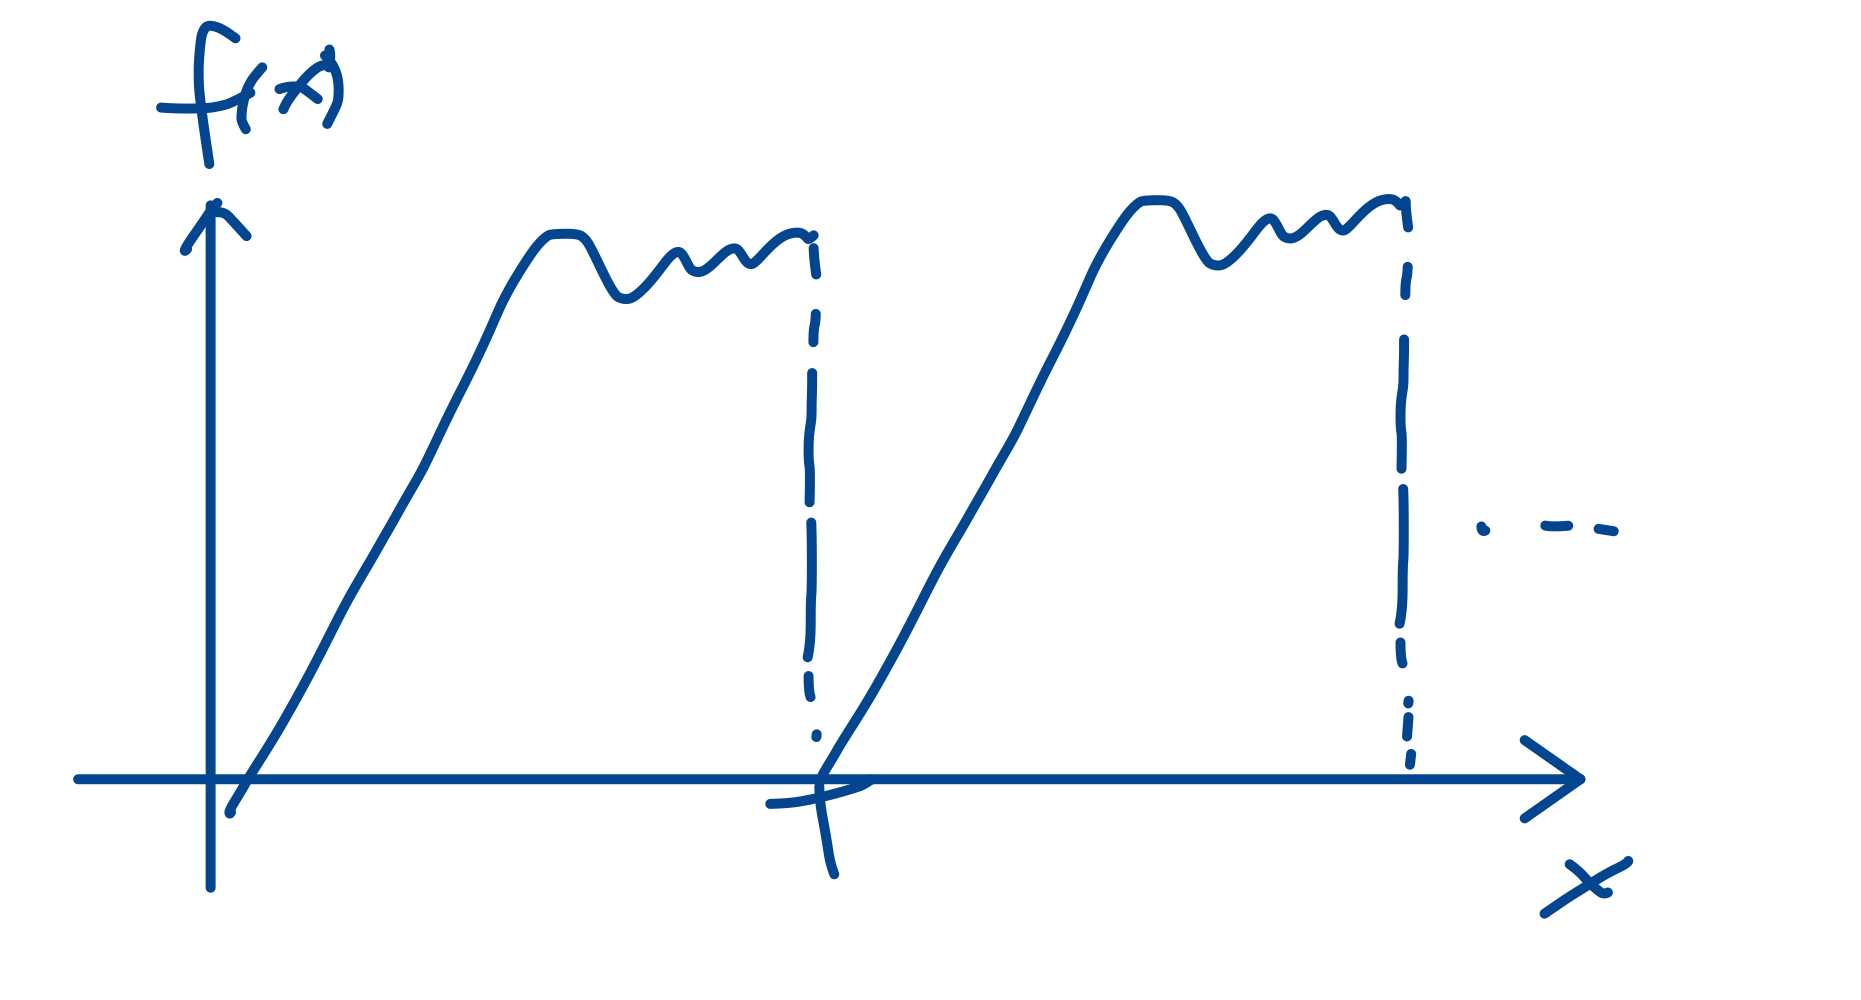
\includegraphics[scale=0.1]{methods1.jpeg}
\end{center}
Consider the set of functions 
\[
    g_n(x) = \cos \left( \frac{n\pi x}{L} \right),\quad h_n(x) = \sin \left( \frac{n\pi x}{L} \right).
\]
They are periodic on $ [0,2L] $ with period 2L.

Recall identities
\[
    \begin{aligned} \cos (A \pm B) &=\cos A \cos B \mp \sin A \sin B \\ \sin (A \pm B) &=\sin A \cos B \pm \cos A \sin B, \text { and so } \\ \cos A \cos B &=\frac{1}{2}[\cos (A-B)+\cos (A+B)] \\ \sin A \sin B &=\frac{1}{2}[\cos (A-B)-\cos (A+B)] \\ \sin A \cos B &=\frac{1}{2}[\sin (A+B)+\sin (A-B)] \end{aligned}
\]
Define an inner product of the set 
\[
    \langle f,g \rangle = \int_{0}^{2L} f(x)g(x)\,\mathrm{d}x.
\]
\begin{proposition}
    With this inner product, $g_n,h_n$ are mutually orthogonal on $ [0,2L) $.
\end{proposition}
\begin{proof}
    Claim that
    \begin{align}
        &\langle h_n,h_m \rangle = \begin{cases}
            L\delta_{nm} &\forall n,m\neq 0\\
            0 & m=0 \lor n=0\\
            \end{cases} \\
            &\langle g_n,g_m \rangle = \begin{cases}
            L \delta_{mn} &n,m\neq 0\\
            2L \delta_{0n} & m=0\\
            \end{cases} \\
            &\langle h_n,g_m \rangle =0
    \end{align}
    \textit{Proof of claim.} Note that for $n\neq m$,
    \begin{align*}
        \langle h_n,h_m \rangle &= \int_{0}^{2L} \sin \frac{n\pi x}{L} \sin \frac{m\pi x}{L} \,\mathrm{d}x\\ 
        &=\int_{0}^{2L} \frac{1}{2}\left( \cos \frac{(n-m)\pi x }{L}-\cos \frac{(n+m)\pi x}{L} \right) \,\mathrm{d}x\\ 
        &= \frac{1}{2} \left[ \frac{L}{(n-m)\pi}\sin \frac{(n-m)\pi x }{L}-\frac{L}{(n+m)\pi} \sin \frac{(n+m)\pi x }{L} \right]_0^{2L}\\ 
        &= \frac{1}{2}\left( \frac{L}{(n-m)\pi}\sin (2\pi(n-m))-\frac{L}{(n+m)\pi} \sin (2\pi(n+m)) \right)\\ 
        &=0.
    \end{align*}
    For $n=m$, 
    \begin{align*}
        \langle h_n,h_m \rangle &= \int_{0}^{2L} \sin^2 \frac{n\pi x}{L} \,\mathrm{d}x\\ 
        &= \int_{0}^{2L} \frac{1-\cos \frac{2n\pi x}{L}}{2} \,\mathrm{d}x\\ 
        &= L.
    \end{align*}
    This proves (1.1). The rest are similar.
\end{proof}
$g_n,h_n$ form a complete orthogonal set, i.e. they span the space of well-behaved periodic functions $ [0,2L) $ and they are linearly independent.

\subsection{Definition of Fourier series}
\begin{definition}
    We can express any well-behaved periodic function of period $2L$ as 
\begin{equation}\label{1.eq.4:FS}
    f(x) = \frac{1}{2}a_0 + \sum_{n=1}^{\infty} a_n \cos \left( \frac{n\pi x}{L} \right)+ \sum_{n=1}^{\infty} b_n \sin \left( \frac{n\pi x}{L} \right)
\end{equation}
where $a_n,b_n$ are constants such that RHS is convergent for all $x$ where $f$ is continuous. At a discontinuity $x$, the Fourier series approaches the midpoint of upper and lower limits at $x$, i.e. 
\[
    \frac{f(x_+)+f(x_-)}{2} = \frac{1}{2}a_0 + \sum_{n=1}^{\infty} a_n \cos \left( \frac{n\pi x}{L} \right)+ \sum_{n=1}^{\infty} b_n \sin \left( \frac{n\pi x}{L} \right).
\]
\end{definition}
Consider $ \langle h_n,f \rangle  $ and substitute in (1.4), we get 
\[
    \int_{0}^{2L} \sin \left( \frac{n \pi x}{L} \right) f(x) \,\mathrm{d}x = \sum_{m=1}^{\infty}Lb_m \delta_{nm} = Lb_n.
\]
Similar for $a_n$. We get
\begin{proposition}
    \begin{equation}
        \begin{aligned}
            &b_{n}=\frac{1}{L} \int_{0}^{2 L} f(x) \sin \left(\frac{n \pi x}{L}\right)\, \rmd x\\ &a_n = \frac{1}{L}\int_{0}^{2L} f(x) \cos \left( \frac{n \pi x}{L} \right) \,\mathrm{d}x
        \end{aligned}
    \end{equation}
\end{proposition}
\begin{note}
    \begin{enumerate}
        \item $a_n$ includes $n=0$ since $ \frac{1}{2}a_0 $ is the average of $f$, i.e.
        \[
            \langle f \rangle = \frac{1}{2L}\int_{0}^{2L} f(x) \,\mathrm{d}x.
        \]
        \item Range of integration can be changed as long as it has length $2L$. We usually consider $ \int_{-L}^{L} $.
        \item Can think of the Fourier series as the decomposition into harmonics. The simplest Fourier series are sines and cosines. e.g. $ \sin (3 \pi x/ L) $ has Fourier series $b_3=1$ and $ b_n=0,n\neq 3 ,a_n=0$.
    \end{enumerate}
\end{note}
\begin{example}[Sawtooth wave]
    Consider $f(x)=x,x\in [-L,L)$ and periodic elsewhere.
    \begin{center}
        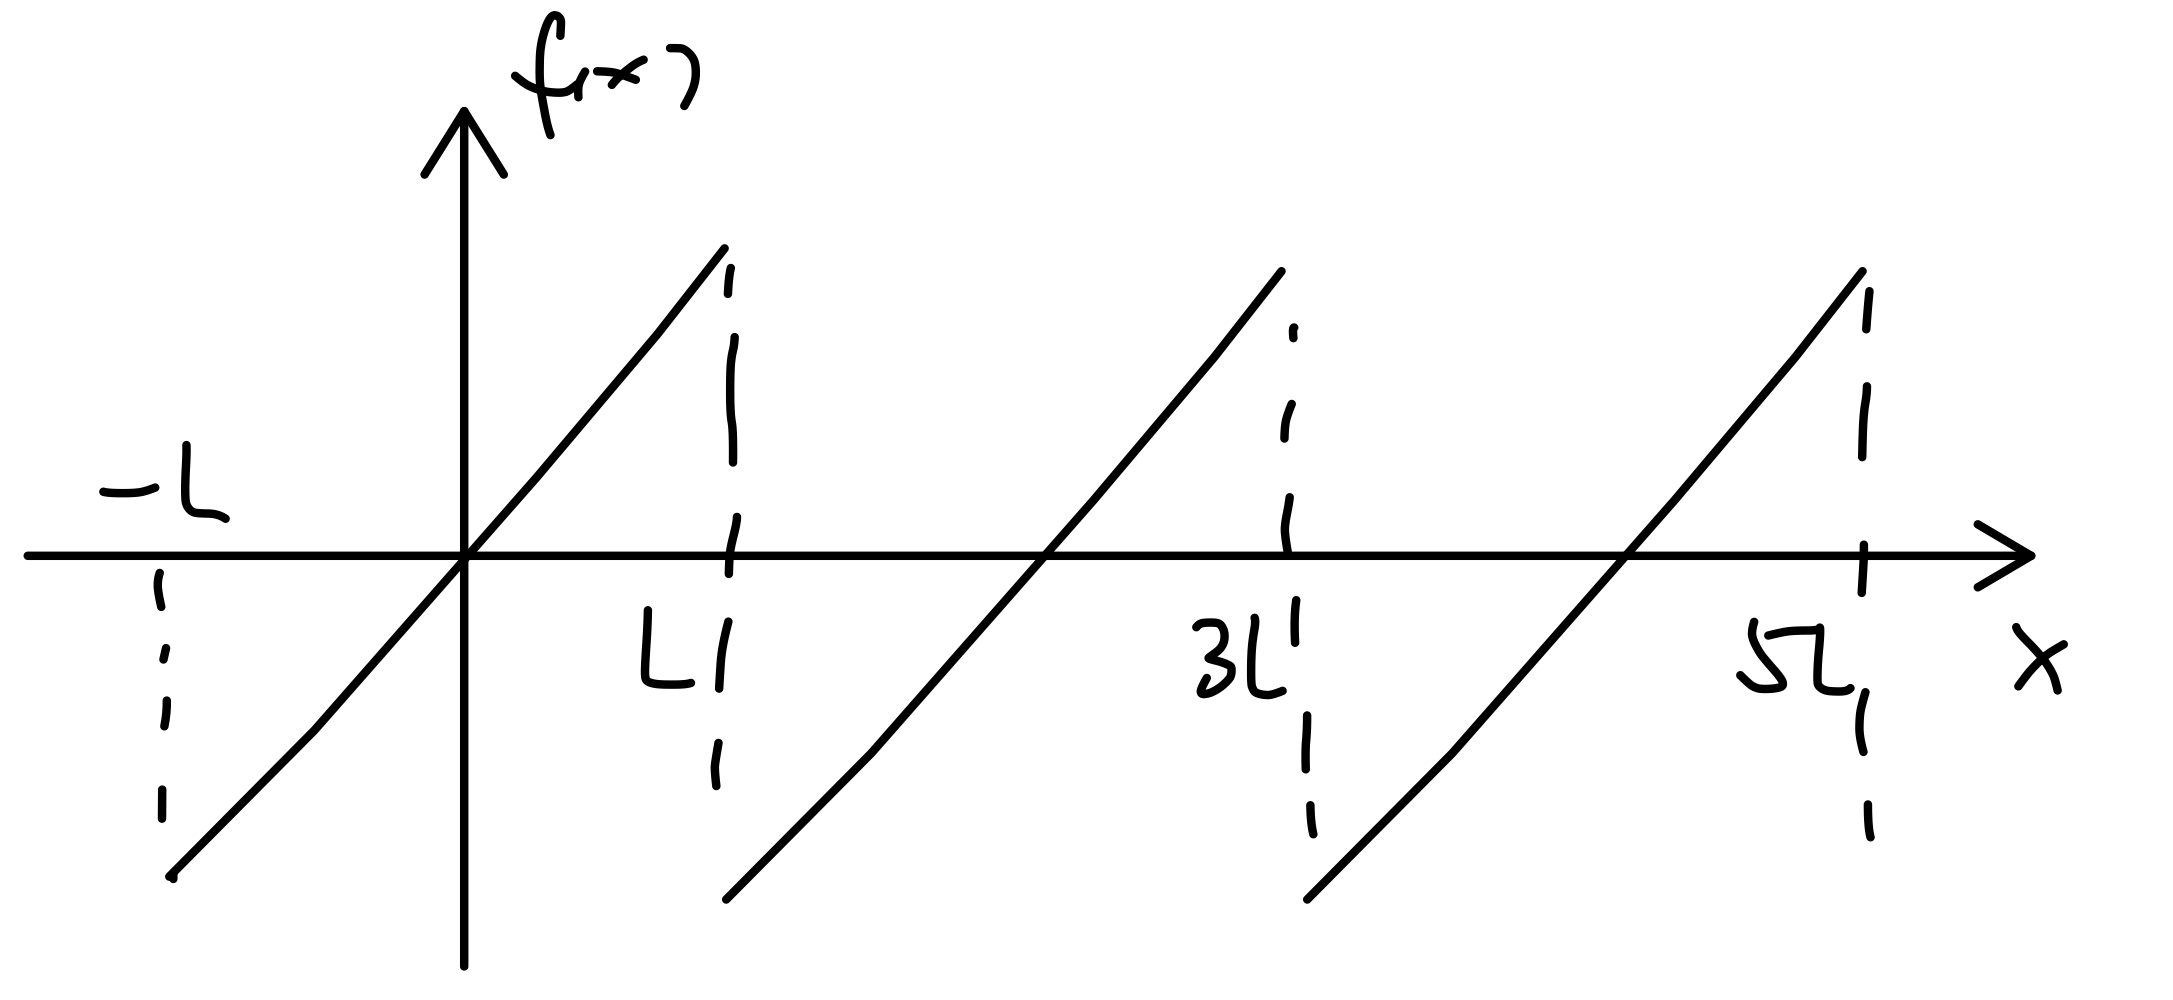
\includegraphics[scale=0.1]{methods2.jpeg}
    \end{center}
    We have 
    \begin{align*}
        a_n &= \frac{1}{L}\int_{-L}^{L} x\cdot \cos \left( \frac{n\pi x}{L} \right) \,\mathrm{d}x=0,\\ 
        b_n &= \frac{2}{L} \int_{0}^{L} x\cdot \sin \left( \frac{n\pi x}{L} \right) \,\mathrm{d}x = \frac{2L}{n\pi }(-1)^{n+1}.
    \end{align*}
    So the Fourier series is 
    \begin{equation}
        f(x) = \frac{2L}{\pi } \sum_{n=1}^{\infty}\frac{(-1)^{n+1}}{n}\sin \left( \frac{n\pi x}{L} \right).
    \end{equation}
\end{example}
\begin{note}
    As $n\to \infty$ in Fourier series,
    \begin{enumerate}
        \item The FS approximation improves (convergent where continuous).
        \item FS $ \to 0 $ at $x=L$, i.e. the midpoint of continuity.
        \item FS has a persistent \textit{overshoot} at $x=L$, which is approximately 9\% and is known as the \textit{Gibbs phenonenon}. See Example Sheet Q5.
    \end{enumerate}
\end{note}

\subsection{The Dirichlet Conditions and Fourier's Theorem}
A natural question is then which functions are allowed to have a proper Fourier series.
Surprisingly, a big, yet hard to precisely characterise, class of functions has a convergent Fourier series that has the desired properties.
This class even includes some classical counterexamples in analysis.
As an applied course, we will just look at some of the sufficient conditions.
\begin{theorem}[Fourier's Theorem]
    If $f$ is a bounded periodic function with period $2L$ with a finite number of minima, maxima, and discontinuities in $[0,2L)$, then its Fourier series converges to $f$ where it is continuous and converges to the average of the two side limits.
\end{theorem}
The conditions in this theorem is known as the Dirichlet conditions.
\begin{note}
    \begin{enumerate}
        \item These conditions are hella weak compared to our conditions for a function to have e.g. a Taylor series.
        However, pathological functions like $1/x,\sin(1/x),1_{\mathbb R\setminus\mathbb Q}(x)$ are excluded from these conditions.
        \item The converse is not true, as $\sin(1/x)$ has a Fourier series we desire.
    \end{enumerate}
\end{note}
\begin{proof}
    See Jeffery \& Jeffery book.
\end{proof}
Another subject of interest is the rate of convergence of a Fourier series.
Perhaps unsurprisingly, it depends on the smoothness of the function.
\begin{theorem}
    If $f(x)$ is $p^{th}$ differentiable but $f^{(p)}$ is not continuous, then its Fourier series converges as $O(n^{-(p+1)})$ as $n\to\infty$.
\end{theorem}
\begin{example}
    \begin{enumerate}
        \item  Consider the square wave
        $$f(x)=\begin{cases}
            1\text{, for $0\le x<1$}\\
            -1\text{, for $-1\le x<0$}
        \end{cases}$$
        That extends periodically with period $2$.
        Then it has a Fourier series
        \begin{equation}
            f(x)=4\sum_{m=1}^\infty\frac{\sin[(2m-1)\pi x]}{(2m-1)\pi}
        \end{equation}
        which, as one can see both from the preceding theorem (with $p=0$) and observation, converges slowly.
        \item Consider the general ``see-saw'' wave
        $$f(x)=\begin{cases}
            x(1-\xi)\text{, for $x\in[0,\xi)$}\\
            \xi(1-x)\text{, for $x\in[\xi,1)$}
        \end{cases}$$
        which extends as an odd periodic function with period $2$.
        This has Fourier series
        \begin{equation}
            f(x)=2\sum_{m=1}^\infty\frac{\sin (n\pi\xi)\sin (n\pi x)}{(n\pi)^2}
        \end{equation}
        which converges with $p=1$ in the preceding theorem.
        In particular, $\xi=1/2$ gives
        $$2\sum_{m=1}^\infty(-1)^{m+1}\frac{\sin[(2m-1)\pi x]}{[(2m-1)\pi]^2}$$
        which can be seen, immediately, that it converges faster than the series in the previous example.
        \item Take $f(x)=x(1-x)/2$ for $x\in[0,1)$ that extends as an odd periodic function with period $2$.
        Then its Fourier series is
        \begin{equation}
            f(x)=4\sum_{m=1}^\infty\frac{\sin[(2m-1)\pi x]}{[(2m-1)\pi]^3}
        \end{equation}
        which has $p=2$.
        \item Take $f(x)=(1-x^2)^2$, then $a_n=O(n^{-4})$.
    \end{enumerate}
\end{example}
Of course, we want to integrate and differentiate a Fourier series term-by-term.
Integration, as one expect, seldom yields problems as it imposed very few restrictions on the function.

And indeed, we are just going to assume we can integrate any Fourier series term-by-term and they guarantee to yield a smoother function, which satisfies the Dirichlet conditions if the original function does.

Differentiation is more problematic when doing it term-by-term.
\begin{example}
    Take the square wave again which is known to have Fourier series
    $$4\sum_{m=1}^\infty\frac{\sin[(2m-1)\pi x]}{(2m-1)\pi}$$
    which, after term-by-term differentiation, yields
    $$4\sum_{m=1}^\infty\cos[(2m-1)\pi x]$$
    which is clearly divergent.
    This is perhaps unsurprising as the original function is not even continuous.
\end{example}
\begin{theorem}
    If $f(x)$ is differentiable and both $f,f^\prime$ satisfy Dirichlet conditions, then we can differentiate the Fourier series of $f$ term-by-term to get the Fourier series of $f^\prime$.
\end{theorem}
\begin{example}
    If we differentiate the see-saw curve with $\xi=1/2$, then we will get an offset of the Fourier series of the square wave with $ \tilde{x}=x+1/2 $.
\end{example}
\subsection{Parseval's Theorem}
There is some interesting relation between the integral of the square of a function and the square of the Fourier coefficients of that function.
If the function is nice enough to have a nice enough Fourier series, then by orthogonality,
\begin{align*}
    \int_0^{2L}f(x)^2\,\mathrm dx&=\int_0^{2L}\left( \frac{a_0}{2}+\sum_{n\ge 1}a_n\cos\frac{n\pi x}{L}+\sum_{n\ge 1}b_n\sin\frac{n\pi x}{L} \right)^2\,\mathrm dx\\
    &=\int_0^{2L}\left( \frac{a_0^2}{4}+\sum_{n\ge 1}a_n^2\cos^2\frac{n\pi x}{L}+\sum_{n\ge 1}b_n^2\sin^2\frac{n\pi x}{L} \right)\,\mathrm dx\\
    &=L\left( \frac{a_0^2}{2}+\sum_{n\ge 1}(a_n^2+b_n^2) \right).
\end{align*}
This is also called the \textit{completeness relation} as the left hand side would be greater than or equal to the right hand side if any basis functions are missing from the series.
This is known as Parseval's Theorem.
\begin{theorem}[Parseval's Theorem]\label{parseval}
    For a nice enough function $f$ with Fourier coefficients $a_n,b_n$, we have
    \begin{equation}
        \int_0^{2L}f(x)^2\,\mathrm dx=L\left( \frac{a_0^2}{2}+\sum_{n\ge 1}(a_n^2+b_n^2) \right).
    \end{equation}
\end{theorem}
\begin{proof}
    Above.
\end{proof}
\begin{example}
    Consider the sawtooth curve with $f(x)=x,x\in[-L,L)$ with period $2L$.
    Then Parseval's Theorem reveals that
    $$\frac{2}{3}L^3=\int_{-L}^Lx^2\,\mathrm dx=L\sum_{n=1}^\infty\frac{4L^2}{n^2\pi^2}=\frac{4L^3}{\pi^2}\sum_{n=1}^\infty\frac{1}{n^2}\implies \sum_{n=1}^\infty\frac{1}{n^2}=\frac{\pi^2}{6}.$$
\end{example}
\begin{remark}
    If we think of the integral of the square as $ \langle f,f \rangle = \left\| f \right\| ^2  $, the $ L^2 $ norm, then Parseval's Theorem can be thought of an analog of Pythagoras' Theorem in this space of functions.
\end{remark}

\subsection{Alternative Fourier Series}
\paragraph{Fourier sines and cosines.}
Consider a function $f:[0,L)\to\mathbb R$.
We can extend $f$ to a periodic function of period $2L$ in two ways:
\begin{enumerate}
    \item We can require the function to be odd, then $a_n=0$ for all $n$ and
    \begin{equation}
        b_n=\frac{2}{L}\int_0^Lf(x)\sin\frac{n\pi x}{L}\,\mathrm dx
    \end{equation}
    and the Fourier series would be $\sum_{n\ge 1}b_n\sin(n\pi x/L)$, which is called a \textit{Fourier sine series}.
    The sawtooth function is an example of this.
    \item We can require the function to be even, then $b_n=0$ for all $n$ and
    \begin{equation}
        a_n=\frac{2}{L}\int_0^Lf(x)\cos\frac{n\pi x}{L}\,\mathrm dx
    \end{equation}
    So the Fourier series is $a_0/2+\sum_{n\ge 1}a_n\cos(n\pi x/L)$.
    This is called a \textit{Fourier cosine series}.
    $f(x)=(1-x^2)^2$ is an example (where $L=1$).
\end{enumerate}
\paragraph{Complex Fourier series.}
The actual thing we want is to represent the Fourier series more neatly in terms of exponentials.
We know that
$$\cos\frac{n\pi x}{L}=\frac{e^{in\pi x/L}+e^{-in\pi x/L}}{2},\sin\frac{n\pi x}{L}=\frac{e^{in\pi x/L}-e^{-in\pi x/L}}{2i}$$
So by writing $c_0=a_0/2$ and
$$c_m=\begin{cases}
    (a_m-ib_m)/2&\text{for $m>0$}\\
    (a_{-m}+ib_{-m})/2&\text{for $m<0$}
\end{cases}$$
we obtain
\begin{equation}
    f(x)=\frac{a_0}{2}+\sum_{n=1}^\infty a_n\cos\frac{n\pi x}{L}+\sum_{n=1}^\infty b_n\sin\frac{n\pi x}{L}=\sum_{m=-\infty}^\infty c_me^{im\pi x/L}
\end{equation}
Equivalently, if we extend our inner product to the complex functions
$$\langle f,g\rangle=\int_{-L}^Lf(x)\overline{g(x)}\,\mathrm dx$$
then we obtain
\begin{equation}
    c_m=\frac{1}{2L}\langle f(x),e^{im\pi x/L}\rangle=\frac{1}{2L}\int_{-L}^Lf(x)e^{-im\pi x/L}\,\mathrm dx
\end{equation}
because of orthogonality
\begin{equation}
    \langle e^{im\pi x/L},e^{in\pi x/L}\rangle= \int_{-L}^{L} e^{-im\pi x/L}e^{in\pi x/L} \,\mathrm{d}x=2L\delta_{mn}
\end{equation}
By thinking them as a set of basis of a space of nice-enough functions in the way we did for $\sin$ and $\cos$.
Parseval's Theorem can then be stated as
$$\int_{-L}^L|f(x)|^2\,\mathrm dx=2L\sum_{n=-\infty}^\infty|c_n|^2$$
\subsection{Some Motivations of Fourier Series}
\begin{definition}
    The complex inner product $\langle\cdot\rangle:\mathbb C^N\times\mathbb C^N\to\mathbb C$ is defined by
    \begin{equation}
        \langle\mathbf{u},\mathbf{v}\rangle=\mathbf{u}^\dagger\mathbf{v}
    \end{equation}
\end{definition}
\begin{definition}
    An $N\times N$  matrix $A$ is \textit{self-adjoint} (or \textit{Hermitian}) if
    $$\forall\mathbf{u},\mathbf{v}\in\mathbb C^N,\langle A\mathbf{u},\mathbf{v}\rangle=\langle\mathbf{u},A\mathbf{v}\rangle.$$
\end{definition}
One can show that this is just saying $A^\dagger=A$.
It can be shown that
\begin{proposition}
    Let $A$ be a self-adjoint matrix. Then the eigenvalues $ \lambda_n $ and eigenvectors $ \bfv_n $ satisfy
    \begin{equation}
        A \bfv_n=\lambda_n\bfv_n
    \end{equation}
    and hence the followings hold:
    \begin{enumerate}[(i).]
        \item All eigenvalues are real for all $n$.
        \item Eigenvectors associated with different eigenvalues are orthogonal with respect to $\langle\cdot\rangle$.
        \item We can rescale to make an orthonormal basis of $\mathbb C^N$ of eigenvectors $\{\mathbf{v}_1,\ldots,\mathbf{v}_N\}$.
    \end{enumerate}
\end{proposition}
\paragraph{Recap of solving linear equations.}
Now, given any $\mathbf{b}$, if we want to solve for $\mathbf{x}$ in
\begin{equation}
    A\mathbf{x}=\mathbf{b}
\end{equation}
then a way to do it is to express $\mathbf{b}=\sum_nb_n\mathbf{v}_n$ and observe that if $\sum_nc_n\mathbf{v}_n$ is a solution then
$$\sum_nb_n\mathbf{v}_n=A\left(\sum_{n=1}^Nc_n\mathbf{v}_n\right)=\sum_{n=1}^Nc_n\lambda_n\mathbf{v}_n$$
where $\lambda_n$ is the eigenvalue associated with $\mathbf{v}_n$.
So if $A$ is nonsingular, then none of the $\lambda_n$ is zero and we can write $c_n=b_n/\lambda_n$ and get the solution
\begin{equation}
    \mathbf{x}=\sum_{n=1}^N\frac{b_n}{\lambda_n}\mathbf{v}_n
\end{equation}
This means we can solve an linear equation if there is a basis consisting of eigenvectors of the matrix.
\paragraph{Analogy to ODEs.}
Consider the differential operator
$$\mathcal Ly=-\frac{\mathrm d^2y}{\mathrm dx^2}$$
and suppose we want to solve
\begin{equation}
    \mathcal{L}y = f(x)\quad \text{subject to}\quad y(0)=y(L)=0.
\end{equation}
The related eigenvalue problem is then $\mathcal L y_n=\lambda_ny_n$ with $y_n(0)=y_n(L)=0$ which has solutions
\begin{equation}\label{1.eq.21}
    y_n(x)=\sin\frac{n\pi x}{L},\quad \lambda_n=\left( \frac{n\pi}{L} \right)^2.
\end{equation}
So we will want to write
\begin{align*}
    &y(x)=\sum_{n=1}^\infty c_n\sin\frac{n\pi x}{L},\\ 
    &f(x)=\sum_{n=1}^\infty b_n\sin\frac{n\pi x}{L},\\ 
    &b_n=\frac{2}{L}\int_0^Lf(x)\sin\frac{n\pi x}{L}\,\mathrm dx,
\end{align*}
assuming convergence.
Then this substitution yields
$$\sum_{n=1}^\infty b_n\sin\frac{n\pi x}{L}=\mathcal Ly=-\frac{\mathrm d^2y}{\mathrm dx^2}\left( \sum_{n=1}^\infty c_n\sin\frac{n\pi x}{L} \right)=\sum_{n=1}^\infty c_n\left( \frac{n\pi}{L} \right)^2\sin\frac{n\pi x}{L}$$
Hence, $c_n=b_n(L/(n\pi))^2$ by orthogonality, so we can get a particular solution of the problem in the form
\begin{equation}
    y(x)=\sum_{n=1}^\infty \frac{b_n}{\lambda_n}y_n = \sum_{n=1}^{\infty}b_n \left( \frac{L}{n\pi} \right)^2 \sin \frac{n\pi x}{L}.
\end{equation}
\begin{example}\label{odd_sq_fourier_ode}
    Consider the problem $ \mathcal{L}y=f(x) $ with $L=1$ and set $f$ to be the odd square wave with $f(x)=1$ for $x\in[0,1)$.
    This has Fourier series
    $$f(x)= 4\sum_{m=1}^\infty\frac{\sin[(2m-1)\pi x]}{(2m-1)\pi}.$$
    So the above discussion instantly yield a solution
    $$y(x)=\sum_{n=1}^\infty \frac{b_n}{\lambda_n}y_n=4\sum_{m=1}^\infty\frac{\sin[(2m-1)\pi x]}{[(2m-1)\pi]^3}$$
    which is the Fourier series of
    \begin{equation}
        y(x)=\frac{x(1-x)}{2}\quad \text{on}\quad[0,1)
    \end{equation}
    extending as an odd periodic function with period $2$.

    Indeed, as one can verifty, if we integrate $\mathcal L y=1$ directly with the appropriate boundary conditions, we can get basically the same solution.
\end{example}
\subsection{A Glimpse into Green's Functions}
In the problem $ \mathcal{L}y=f(x) $, fix $L=1$ and consider an odd function $f$.
We have
\begin{align}
    y(x)&=\sum_{n=1}^\infty\frac{b_n}{\lambda_n}\sin(\pi x)\nonumber\\
    &=\sum_{n=1}^\infty\frac{2}{(n\pi)^2}\left(\int_0^1f(\xi)\sin(n\pi\xi)\,\mathrm d\xi\right)\sin(n\pi x)\nonumber\\
    &=\int_0^12\sum_{n=1}^\infty\frac{\sin(n\pi x)\sin(n\pi\xi)}{(n\pi)^2}f(\xi)\,\mathrm d\xi\tag{Assume swapping limits}\\
    &=\int_0^1G(x,\xi)f(\xi)\,\mathrm d\xi
\end{align}
where
\begin{equation}
    G(x,\xi)=2\sum_{n=1}^\infty\frac{\sin(n\pi x)\sin(n\pi\xi)}{(n\pi)^2}.
\end{equation}
It is exactly the general see-saw wave
\begin{equation}
    G(x,\xi)=\begin{cases}
        x(1-\xi)\text{, for $x\in[0,\xi)$}\\
        \xi(1-x)\text{, for $x\in[\xi,1)$}
    \end{cases}
\end{equation}
This is the \textit{Green's function} for this ODE $-\rmd^2 y/\rmd x^2 =f(x)$.
One can actually solve this integral and get what we got in Example \ref{odd_sq_fourier_ode}.

\section{Sturm-Liouville Theory}
\subsection{Review of Second-Order Linear ODEs}
For a general inhomogeneous ODE $\mathcal Ly=f(x)$ where
\begin{equation}
    \mathcal Ly=\alpha(x)\frac{\mathrm d^2y}{\mathrm dx^2}+\beta(x)\frac{\mathrm dy}{\mathrm dx}+\gamma(x)y
\end{equation}
In general, the homogeneous equation
\begin{equation}
    \mathcal Ly=0
\end{equation}
has two linearly independent solutions $y_1,y_2$.
The complementary function
\begin{equation}
    y_c(x)=Ay_1+By_2
\end{equation}
for constants $A,B$ is then the general solution to $\mathcal Ly=0$ by linearity.

For the inhomogeneous problem 
\begin{equation}
    \mathcal Ly=f(x)
\end{equation}
If we can find a particular solution (aka particular integral) $y_p$ to $\mathcal Ly=f$, then
\begin{equation}
    y=y_p+y_c=y_p+Ay_1+By_2
\end{equation}
for $A,B$ constants is the general solution to $\mathcal Ly=f$ again by linearity.
Two pieces of boundary data is then needed to determine the constants $A,B$.

There are several types of boundary conditions.
\begin{itemize}
    \item The Dirichlet condition of specifying the function's value at the endpoints, \item The Neumann condition of specifying the derivative's values at the endpoints.
    \item Mixed conditions of above.
\end{itemize}

The sort of conditions we often consider are homogeneous conditions, i.e. the function vanishes at the endpoints.
The reason of it is that it allows the \textit{superposition} of solutions in a linear DE.
What if we come across a inhomogeneous condition?
We can use the complementary solution to cancel stuff out.

Sometimes, we specify initial data of the function and its derivative as boundary conditions.

Another matter of interest is the general eigenvalue problem.
To solve $\mathcal Ly=f$ using eigenvalue decompositions like we did previously, we must first solve (subject to boundary conditions) the related eigenvalue problem
\begin{equation}
    \mathcal Ly=\alpha(x)\frac{\mathrm d^2y}{\mathrm dx^2}+\beta(x)\frac{\mathrm dy}{\mathrm dx}+\gamma(x)y=-\lambda\rho(x)y
\end{equation}
where $\rho$ is nonegative.
This form often occurs after seperation of variables in a PDE.
\subsection{Self-Adjoint Operators}
\begin{definition}
    For two functions $f,g:[a,b]\to\mathbb C$ we define their inner product to be
    $$\langle f,g\rangle=\int_a^bf^*(x)g(x)\,\mathrm dx$$
\end{definition}

\begin{definition}[Sturm-Liouville form]
    An ODE $ \mathcal{L}y=f(x) $ can be written as the \textit{Sturm-Liouville form} if $ \mathcal{L} $ can be written as
    \[
        \mathcal{L}y=-(py')'+qy,
    \]
    where $ p,q$ are functions, and the ODE $ \mathcal{L}y=f(x) $ can be written as 
    \begin{equation}
        \mathcal{L}y=-(py')'+qy=\lambda w y,
    \end{equation}
    where $w$ is a nonnegative weight function.
\end{definition}

We can guarantee to rewrite the original eigenvalue problem into the Sturm-Liouville form.

\paragraph{Integrating factor} How to convert a second order linear ODE to this form?
Simply multiply the diffential equation by an integrating factor $F$ that will be specified later and we can write
\begin{align*}
    &F \alpha y''+F \beta y'+ F \gamma y = -\lambda F \rho y\\ 
    \implies&\frac{\mathrm d}{\mathrm dx}(F\alpha y^\prime)-F^\prime\alpha y^\prime-F\alpha^\prime y^\prime+F\beta y^\prime+F\gamma y=-\lambda F\rho y.
\end{align*}
So to eliminate the $y^\prime$ terms, we set
\begin{equation}
    F^\prime\alpha y^\prime+F\alpha^\prime y^\prime-F\beta y^\prime=0 \Longrightarrow  F(x)=\exp\left(\int\frac{\beta-\alpha^\prime}{\alpha}\,\mathrm dx\right)
\end{equation}
which reduced the equation to
$$(F\alpha y^\prime)^\prime+F\gamma y=-\lambda F\rho y \Longleftrightarrow -(py')'+qy=\lambda w y,$$
setting $p=F\alpha,q=-F\gamma$ and $w=F\rho\ge 0$.
\begin{example}
    Consider the Hermite equation that appears in quantum mechanics
    $$y^{\prime\prime}-2xy^\prime+2ny=0$$
    Then $\alpha=1,\beta=-2x,\gamma=0,\lambda\rho=2n$, so the above procedure translates this to the Sturm-Liouville form
    \begin{equation}\label{2.eq.9}
        \mathcal Ly=(-e^{-x^2}y^\prime)^\prime=2ne^{-x^2}y
    \end{equation}
\end{example}
\subsubsection*{Boundary conditions}

\begin{definition}[Self-adjoint operators]
    Let $\mathcal L:C\to C$ be an operator, where $C$ on a class of functions $[a,b]\to\mathbb C$ equipped with the inner product above.
    $\mathcal L$ is \textit{self-adjoint} if $\langle y_1,\mathcal Ly_2\rangle=\langle\mathcal Ly_1,y_2\rangle$ for any $y_1,y_2\in C$. Equivalently,
    \begin{equation}
        \int_{a}^{b} y_1^*(x)\mathcal{L}y_2(x) \,\mathrm{d}x = \int_{a}^{b} (\mathcal{L}y_1(x))^* y_2(x) \,\mathrm{d}x
    \end{equation}
\end{definition}

If we let $\mathcal L$ be the operator in the Strum-Liouville form, then
\begin{align}
    \langle y_1,\mathcal Ly_2\rangle-\langle\mathcal Ly_1,y_2\rangle&=\int_a^b[-y_1(py_2^\prime)^\prime+y_1qy_2+y_2(py_1^\prime)^\prime-y_2qy_1]\,\mathrm dx\nonumber\\
    &=\int_a^b[-y_1(py_2^\prime)^\prime+y_2(py_1^\prime)^\prime]\,\mathrm dx\nonumber\\
    &=\int_a^b[-(y_1(py_2^\prime)^\prime+y_1^\prime py_2^\prime)+(y_2(py_1^\prime)^\prime+y_2^\prime py_1^\prime)]\,\mathrm dx\nonumber\\
    &=\int_a^b[-(py_1y_2^\prime)^\prime+(py_1^\prime y_2)^\prime]\,\mathrm dx\nonumber\\
    \implies \langle y_1,\mathcal Ly_2\rangle-\langle\mathcal Ly_1,y_2\rangle&=[-py_1y_2^\prime+py_1^\prime y_2]_a^b
\end{align}
So for this operator to be self-adjoint, we need some good enough boundary conditions so that enough stuff vanishes.
This includes homogeneous boundary condition $y(a)=y(b)=0$ or $y^\prime(a)=y^\prime(b)=0$ or mixed $y+ky^\prime=0$ etc.

We say a Sturm-Liouville problem is \textit{regular} if the boundary conditions are homogeneous.
Periodic boundary conditions also work, where we can take $y(a)=y(b)$ and the derivatives are specified (or periodic) at the boundary.
There can also be singular points of this ODE, where $p(a)=p(b)=0$.
We can have combinations of above too.

\subsection{Properties of Self-Adjoint Operators}
Analogous to the finite dimensional case, we have
\begin{theorem}\label{self-adjoint}
    For a sufficiently nice self-adjoint operator $\mathcal L$ on a sufficiently nice space of functions:
    \begin{enumerate}[(a)]
        \item Eigenvalues of $\mathcal L$ are real.
        \item Eigenfunctions of it with different eigenvalues are orthogonal with respect to the weight $w$.
        \item We can take the eigenfunctions as a set of basis for the function space, just like Fourier series.
    \end{enumerate}
\end{theorem}
\begin{proof}[Proof of (a)]
    Given
    \begin{equation}\label{2.eigenproblem}
        \mathcal Ly=\lambda wy
    \end{equation}
    taking complex conjugate gives $\mathcal Ly^*=\lambda^*wy^*$.
    Hence as $\mathcal L$ is self-adjoint,
    $$0=\int_a^b(y^*\mathcal Ly-y\mathcal Ly^*)\,\mathrm dx=(\lambda-\lambda^*)\int_a^bw|y|^2\,\mathrm dx$$
    which means $\lambda=\lambda^*$, so $\lambda$ is real.
\end{proof}
If $\lambda$ is non-degenerate (simple), i.e. it has a one-dimensional eigenspace, then $y$ is guaranteed to be real.
Even if it has dimension $2$ (not more because the ODE is second order), we can still find two real functions as basis of the eigenspace. Hence from now on, we assume the eigenfunctions to be real.

Also, by considering $u\mathcal Lv-v\mathcal Lu=(-p(uv^\prime-u^\prime v))^\prime$, one can show that a regular Sturm-Liouville problem always has all eigenvalues simple.

\begin{proof}[Proof of (b)]
    Suppose $\mathcal Ly_m=\lambda_mwy_m$ and $\mathcal Ly_n=\lambda_nwy_n$, then
    \begin{equation}\label{2.eq.13}
        0=\int_a^by_n\mathcal Ly_m-y_m\mathcal Ly_n\,\mathrm dx=(\lambda_m-\lambda_n)\int_a^bwy_ny_m\,\mathrm dx
    \end{equation}
    But $\lambda_m$ and $\lambda_n$ are distinct.
    The claim follows.
\end{proof}

\begin{definition}
    The inner product of $y_1,y_2:[a,b]\to\mathbb C$ with respect to weight $w:[a,b]\to\mathbb R_{\ge 0}$ is
    \begin{equation}
        \langle f,g\rangle_w=\int_a^bwf^*g\,\mathrm dx=\langle wf,g\rangle=\langle f,wg\rangle
    \end{equation}
\end{definition}

So the orthogonality in (\ref{2.eq.13}) becomes 
\begin{equation}
    \langle y_n,y_m \rangle _w = 0,\quad \forall n\neq m.
\end{equation}

\begin{remark}
    Watch the weight!
\end{remark}

As an aside, we do not really need the weight function in order to formulate Sturm-Liouville theory, since we can do the transformation $\tilde{y}=\sqrt{w}y$ and replace $\mathcal Ly$ by $(1/\sqrt{w})\mathcal L(\tilde{y}/\sqrt{w})$.
Yet the analytic property is generally simpler if we keep $w$.
\begin{example}
    For the Hermite equation \ref{2.eq.9}, we can eliminate $ w $ with $ \tilde{y}=e^{-x^2/2}y $ to find 
    \[
        \tilde{\mcL} = -\tilde{y}''+(x^2-1)\tilde{y}=2n \tilde{y}.
    \]
\end{example}
\subsection{Eigenfunction expansion}
Completeness ((c) in theorem \ref{self-adjoint}) implies we can approximate any well-behaved $f(x)$ on $ [a,b] $ by the series 
\begin{equation}
    f(x)=\sum_{n=1}^\infty a_ny_n(x)
\end{equation}
where $y_n$ is a set of eigenfunctions of some self-adjoint operator.
To find the coefficients $a_n$, we can use the orthogonality (\ref{2.eq.13}) to get
\[
    \int_{a}^{b} w(x)y_m(x)\cdot f(x) \,\mathrm{d}x = \sum_{n=1}^{\infty}a_n \int_{a}^{b} wy_ny_m \,\mathrm{d}x = a_m\int_a^bwy_m^2\,\mathrm dx
\]
Hence 
\begin{equation}\label{2.eq.17}
    a_n=\left(\int_a^bwy_nf\,\mathrm dx\middle)\right/\left(\int_a^bwy_n^2\,\mathrm dx\right)
\end{equation}
It's a common practice not to normalise the eigenfunctions as it is not really always clean.
Of course, if we want, we can always write down
\[
    Y_n=y_n\left/\sqrt{\int_a^bwy_n^2\,\mathrm dx}\right.
\]
So that 
\begin{equation}
    \langle Y_n,Y_m \rangle =\delta_{nm}
\end{equation}
are orthonormal with 
\[
    f(x) = \sum_{n=1}^{\infty}A_nY_n(x)\quad \text{and}\quad A_n = \int_{a}^{b} w(x)Y_n(x)f(x) \,\mathrm{d}x
\]
\begin{example}
    Recall the particular operator already in Sturm-Liouville form $\mathcal Ly=-y^{\prime\prime}$, then (with appropriate boundary conditions) we can easily get the eigenvalues $\lambda_n=(n\pi/L)^2$ and eigenfunctions being the trigonometrics.
    This just reproduces the Fourier series.
\end{example}
\subsection{Completeness and Parseval's Identity}
We expand
\begin{align*}
    &\int_a^bw\left( f(x)-\sum_{n=1}^\infty a_ny_n \right)^2\,\mathrm dx\\
    =&\int_a^bw\left( f^2-2f\sum_{n=1}^\infty a_ny_n+\sum_{n=1}^\infty a_n^2y_n^2 \right)\,\mathrm dx\tag{Last term by orthogonality} \\    
    =&\int_a^bwf^2\,\mathrm dx-\sum_{n=1}^\infty a_n^2\int_a^bwy_n^2\,\mathrm dx\tag{By \ref{2.eq.17}}
\end{align*}
If the eigenfunctions are complete, then the series expansion converges, and thus the above expansion is 0 and 

\begin{align}\label{2.eq.19}
    \int_a^bwf^2\,\mathrm dx&=\sum_{n=1}^\infty a_n^2\int_a^bwy_n^2\,\mathrm dx\\ 
    &=\sum_{n=1}^\infty A_n^2\text{ for unit normal $Y_n$}\nonumber
\end{align}
Note that $\int_a^bwy_n^2\,\mathrm dx$ becomes $L$ for Fourier series.

If some of the eigenfunctions are missing from the series, then this gives
$$\int_a^bwf^2\,\mathrm dx\ge\sum_{n=1}^\infty A_n^2$$
This is known as Bessel's Inequality.
\paragraph{Calculating the error}
Consider the partial sums $\sum_{n\le N}a_ny_n$, then we shall have
\begin{equation}\label{2.eq.20}
    f(x) = \lim_{N \to \infty} S_N(x)
\end{equation}
Convergence is defined in terms of the \textit{mean square error}
\[
    \epsilon_N=\int_a^bw[f(x)-S_N(x)]^2\,\mathrm dx\to 0,N\to\infty
\]
This global definition of convergence in mean is not the pointwise convergence of Fourier series, which converges to all the continuous points of $f$.

An interesting question is that, while we know (maybe) the series converges as we want, if we truncate the sequence in some $N$, would the coefficients $\{a_n\}_{n\le N}$ provide the best approxmation (with respect to the error defined in this way) of that particular partial sum, or a different set of partial coefficient will yield a better result?
The answer is yes. 
\begin{claim}
    The error in partial sums (\ref{2.eq.20}) is minimised by $a_n$ in (\ref{2.eq.19}) for $ N= \infty  $ expansion.
\end{claim}
\begin{proof}
    Differentiate wrt $a_n$ gives
    $$\frac{\partial\epsilon_N}{\partial a_n}=-2\int_a^bwy_n\left( f-\sum_{k=1}^Na_ky_k \right)\,\mathrm dx=-2\int_a^bwfy_n-a_nwy_n^2\,\mathrm dx$$
    which is zero when $a_n$ is of the expression in (\ref{2.eq.17}).
    We can see it is indeed a minimum by observing that
    $$\frac{\partial^2\epsilon_N}{\partial a_n^2}=2\int_a^bwy_n^2\,\mathrm dx\ge 0$$
    This answers our question.
\end{proof}
\subsection{Legendre's Equation}
Take the usual spherical polar coordinate
$$\begin{cases}
    x=r\sin\theta\cos\phi\\
    y=r\sin\theta\sin\phi\\
    z=r\cos\theta
\end{cases}$$
where Laplace's equation $\nabla^2 u=0$ translates to
$$\frac{1}{r^2}\frac{\partial}{\partial r}\left( r^2\frac{\partial u}{\partial r} \right)+\frac{1}{r^2\sin\theta}\frac{\partial}{\partial\theta}\left( \sin\theta\frac{\partial u}{\partial\theta} \right)+\frac{1}{r^2\sin^2\theta}\frac{\partial^2u}{\partial\phi^2}=0$$
Seperation of variables $u=R(r)\Theta(\theta)\Phi(\phi)$ then gives
$$\frac{1}{\sin\theta}(\Theta^\prime\sin\theta)^\prime+\left( K-\frac{m^2}{\sin^2\theta} \right)\Theta=0$$
where $K,m$ are constants which essentially makes it an eigenvalue problem.

Now the transformation $x=\cos\theta\in[-1,1]$ and renaming $\Theta$ as $y$ then gives Legendre's Equation
\begin{equation}\label{2.eq.21:legendre}
    (1-x^2)y^{\prime\prime}-2xy^\prime+\lambda y=0
\end{equation}
where $\lambda$ is a constant which is again intepreted as an eigenvalue.
This is already in Strum-Liouville form by taking $p=1-x^2,q=0,w=1$.
Now $p=1-x^2$ vanishes at the boundary $\pm 1$, so this equation has to be self-adjoint.
We assume that $y$ is bounded near the boundary. (Regular singular point)

We now seek a power series solution to the problem.
If we set
$$y=\sum_{n=0}^\infty c_nx^n$$
Then substitution gives 
\begin{align}\label{2.eq.22}
    &(1-x^2)\sum_n n(n-1)c_nx^{n-2}-2x \sum_n c_n x^{n-1} + \lambda \sum_n c_n x^n=0\nonumber\\
    \Longrightarrow & (n+2)(n+1)c_{n+2}-n(n-1)c_n-2nc_n+\lambda c_n=0\nonumber\\ 
    \implies &c_{n+2}=\frac{n(n+1)-\lambda}{(n+1)(n+2)}c_n
\end{align}
Specifying $c_0,c_1$ gives 2 independent solution near $ x=0 $:
\begin{align*}
    y_{\text{even}}&=c_0\left( 1+\frac{(-\lambda)}{2!}x^2+\frac{(6-\lambda)(-\lambda)}{4!}x^4+\cdots \right)\\
    y_{\text{odd}}&=c_1\left( x+\frac{2-\lambda}{3!}x^3+\cdots \right)
\end{align*}
Note that $c_{n+2}/c_n\to 1$, so the both series has radius of convergence $1$ but they diverges at $x=\pm 1$.

These series may not be infinite.
If $\lambda=l(l+1)$ for some $l\in\mathbb N$, then one of these two series will terminate and give a polynomial solution.
These polynomials are called \textit{Legendre polynomials} $P_l(x)$ which are eigenfunctions of the Legendre equation (\ref{2.eq.21:legendre}).

Conventionally we normalise $P_l$ by requiring $P_l(1)=1$.
One can check that this restricts $P_l([-1,1])\subset [-1,1]$ and $|P_l(-1)|=1$.
By calculation we have
\begin{align*}
    P_{0}(x)&=1\\ 
    P_{1}(x)&=x\\ 
    P_{2}(x)&=\frac{1}{2}\left(3 x^{2}-1\right)\\ 
    P_{3}(x)&=\frac{1}{2}\left(5 x^{3}-3 x\right)
\end{align*}
Note that 
\begin{enumerate}
    \item $P_l$ has $l$ roots in $[-1,1]$.
    \item $P_l$ is odd if $l$ is odd, and even when $l$ is even.
\end{enumerate}

\subsection{Properties of Legendre polynomials}
Since Legendre polynomials come from a self-adjoint operator, they must have certain conditions, such as orthogonality.
\begin{proposition}
    For \( n \neq m \), $\displaystyle \int_{-1}^1 P_n P_m \dd{x} = 0$. 
\end{proposition}
They are also normalisable,
\begin{proposition}
    $\displaystyle 
	\int_{-1}^1 P_n^2 \dd{x} = \frac{2}{2n+1}$
\end{proposition}
We can prove this with Rodrigues' formula:
\begin{proposition}
    $\displaystyle P_n(x) = \frac{1}{2^n n!} \qty( \dv{x} )^n (x^2 - 1)^n$ 
\end{proposition}
Alternatively we could use a generating function:
\begin{proposition}
    \begin{align*}
        \sum_{n=0}^\infty P_n(x) t^n = \frac{1}{\sqrt{1 - 2xt + t^2}} & = 1 + \frac{1}{2}\qty(2xt - t^2) + \frac{3}{8}\qty(2xt - t^2)^2 + \dots \\
                                                                      & = 1 + xt + \frac{1}{2}\qty(3x^2 - 1)t^2 + \dots
    \end{align*}
\end{proposition}
There are some useful recursion relations.
\begin{proposition}\
    \begin{enumerate}[(i)]
        \item $ \ell(\ell + 1) P_{\ell + 1} = (2 \ell + 1) x P_\ell(x) - \ell P_{\ell - 1}(x) $
        \item $\displaystyle (2\ell + 1)P_\ell(x) = \dv{x} \qty[ P_{\ell + 1}(x) - P_{\ell - 1}(x) ]$.
    \end{enumerate}
\end{proposition}

\subsection{Eigenfunction expansion}
Any (well-behaved) function on \( [-1,1] \) can be expressed as
\[
	f(x) = \sum_{\ell = 0}^\infty a_\ell P_\ell(x)
\]
where
\[
	a_\ell = \frac{2\ell + 1}{2} \int_{-1}^1 f(x) P_\ell(x) \dd{x}
\]
with no boundary conditions (e.g.\ periodicity conditions) on \( f \).

\subsection{S-L Theory on inhomogeneous ODEs}

\paragraph{Solve ODEs using SL theory} Consider the problem
\[
	\mathcal L y = f(x) \equiv w(x) F(x)
\]
on \( x \in [a,b] \) assuming homogeneous boundary conditions.
Given eigenfunctions \( y_n(x) \) satisfying \( \mathcal L y_n = \lambda_n w y_n \), we wish to expand this solution as
\[
	y(x) = \sum_n c_n y_n(x)
\]
and
\[
	F(x) = \sum_n a_n y_n(x)
\]
where \( a_n \) are known and \( c_n \) are unknown:
\[
	a_n = \frac{\int_a^b w F y_n \dd{x}}{\int_a^b w y_n^2 \dd{x}}
\]
Substituting,
\[
	\mathcal L y = \mathcal L \sum_n c_n y_n = w \sum_n c_n \lambda_n y_n = w \sum_n a_n y_n
\]
By orthogonality,
\[
	c_n \lambda_n = a_n \implies c_n = \frac{a_n}{\lambda_n}
\]
In particular,
\[
	y(x) = \sum_{n=1}^\infty \frac{a_n}{\lambda_n}y_n(x)
\]
\paragraph{Generalisation} Driving force often induces a linear response term \( \widetilde\lambda w y \).
\[
	\mathcal L y - \widetilde \lambda w y = f(x)
\]
where \( \widetilde \lambda \neq \lambda \). 
The solution becomes
\[
	y(x) = \sum_{n=1}^\infty \frac{a_n}{\lambda_n - \widetilde \lambda} y_n(x)
\]

\subsection{Integral solutions and Green's function}
Recall that
\[
	y(x) = \sum_{n=1}^\infty \frac{a_n}{\lambda_n} y_n(x) = \sum_n \frac{y_n(x)}{\lambda_n  N_n} \int_a^b w(\xi) F(\xi) y_n(\xi) \dd{\xi}
\]
where
\[
	N_n = \int w y_n^2 \dd{x}
\]
This then gives
\[
	y(x) = \int_a^b \underbrace{\sum_{n=1}^\infty \frac{y_n(x) y_n(\xi)}{\lambda_n N_n}}_{G(x,\xi)} \underbrace{w(\xi) F(\xi)}_{f(\xi)} \dd{\xi} = \int_a^b G(x;\xi) f(\xi) \dd{\xi}
\]
where
\[
	G(x,\xi) = \sum_{n=1}^\infty \frac{y_n(x) y_n(\xi)}{\lambda_n N_n}
\]
is the eigenfunction expansion of the \textbf{Green's function}.
Note that the Green's function does not depend on \( f \), but only on \( \mathcal L \) and the boundary conditions.
In this sense, it acts like an inverse operator
\[
	\mathcal L^- \equiv \int \dd{\xi} G(x,\xi)
\]
analogously to how \( Ax = b \implies x = A^{-1} b \) for matrix equations.

\clearpage

\part{PDEs on bounded domains}
\section{The Wave Equation}
\subsection{Waves on an elastic string: physical derivation}
Consider a small displacement \( y(x,t) \) on a stretched string with fixed ends at \( x = 0 \) and \( x = L \), that is, with boundary conditions \( y(0,t) = y(L,t) = 0 \).
We can determine the string's motion for specified initial conditions \( y(x,0) = p(x) \) and \( \pdv{y}{t}(x,0) = q(x) \).

We derive the equation of motion governing the motion of the string by balancing forces on a string segment \( (x,x+\delta x) \) and take the limit as \( \delta x \to 0 \).
Let \( T_1 \) be the tension force acting to the left at angle \( \theta_1 \) from the horizontal.
Analogously, let \( T_2 \) be the rightwards tension force at angle \( \theta_2 \).
We assume at any point on the string that \( \abs{\pdv{y}{x}} \ll 1 \), so the angles of the forces are small.
In the \( x \) dimension,
\[
	T_1 \cos \theta_1 = T_2 \cos \theta_2 \implies T_1 \approx T_2 = T
\]
So the tension \( T \) is constant up to an error of order \( O\qty(\abs{\pdv{y}{x}
}^2) \).
In the \( y \) dimension, since \( \theta \) are small,
\[
	F_T = T_2 \sin \theta_2 - T_1 \sin \theta_1 \approx T \qty(\eval{\pdv{y}{x}}_{x + \delta x} - \eval{\pdv{y}{x}}_x) \approx T \pdv[2]{y}{x} \delta x
\]
By \( F = ma \),
\[
	F_T + F_g = (\mu \delta x) \pdv[2]{y}{t} = T \pdv[2]{y}{x} \delta x - g \mu \delta x
\]
where \( F_g \) is the gravitational force and \( \mu \) is the linear mass density.
We define the wave speed as
$ c = \sqrt{T/\mu} $
and find
\[
	\pdv[2]{y}{t} = \frac{T}{\mu} \pdv[2]{y}{x} - g = c^2 \pdv[2]{y}{x}-g
\]
We often assume gravity is negligible to produce the pure wave equation
\[
	\frac{1}{c^2} \pdv[2]{y}{t} = \pdv[2]{y}{x} 
\]

\subsection{Separation of variables}

Consider a separable form:
\[
	y(x,t) = X(x) T(t)
\]
Substituting into the wave equation,
\[
	\frac{1}{c^2} \ddot y = y'' \implies \frac{1}{c^2} X \ddot T = X'' T
\]
Then
\[
	\frac{1}{c^2}\frac{\ddot T}{T} = \frac{X''}{X}
\]
However, \( \frac{\ddot T}{T} \) depends only on \( t \) and \( \frac{X''}{X} \) depends only on \( x \).
Thus, both sides must be equal to some \textbf{separation constant} \( -\lambda \).
\[
	\frac{1}{c^2}\frac{\ddot T}{T} = \frac{X''}{X} = -\lambda \implies X'' + \lambda X = 0;\quad \ddot T + \lambda c^2 T = 0
\]

\subsection{Boundary conditions and normal modes}

First look at the spatial part of the solution.

One of \( \lambda > 0, \lambda < 0, \lambda = 0 \) must be true.
The boundary conditions restrict the possible \( \lambda \).
\begin{enumerate}[align=left]
	\item[(1) \( \lambda < 0 \)] Take \( \chi^2 = -\lambda \).
	      Then,
	      \[
		      X(x) = Ae^{\chi x} + Be^{-\chi x} = \tilde{A} \cosh (\chi x) + \tilde{B} \sinh (\chi x)
	      \]
	      The boundary conditions are \( x(0) = x(L) = 0 \), so only the trivial solution is possible: \( \tilde{A} = \tilde{B} = 0 \).
	\item[(2) \( \lambda = 0 \)] Then
	      \[
		      X(x) = Ax + B
	      \]
	      Again, the boundary conditions impose \( A = B = 0 \) giving only the trivial solution.
	\item[(3) \( \lambda > 0 \)]
	      \[
		      X(x) = A \cos \qty(\sqrt{\lambda} x) + B \sin \qty(\sqrt{\lambda} x)
	      \]
	      The boundary conditions give
	      \[
		      A = 0,\quad B \sin \qty(\sqrt{\lambda} L) = 0 \implies \sqrt{\lambda} L = n \pi
	      \]
\end{enumerate}
The following are the eigenfunctions and eigenvalues.
\[
	X_n(x) = B_n \sin \frac{n \pi x}{L};\quad \lambda_n = \qty(\frac{n \pi}{L})^2
\]
These are also called the \textbf{normal modes} of the system.
The spatial shape in \( x \) does not change in time, but the amplitude may vary.
The \textbf{fundamental mode}, or \textbf{first harmonic}, is the lowest frequency of vibration, given by
\[
	n = 1 \implies \lambda_1 = \frac{\pi^2}{L^2}
\]
The \textbf{second mode}, or \textbf{overtone}, is the first overtone, and is given by
\[
	n = 2 \implies \lambda_2 = \frac{4\pi^2}{L^2}
\]
and so on. 

\subsection{Initial conditions and temporal solutions}
Substituting \( \lambda_n \) into the time ODE,
\[
	\ddot T + \frac{n^2 \pi^2 c^2}{L^2}T = 0
\]
Hence,
\[
	T_n(t) = C_n \cos \left(\frac{n \pi c t}{L}\right) + D_n \sin \left(\frac{n \pi c t}{L}\right)
\]
Therefore, a specific solution of the wave equation satisfying the boundary conditions is (absorbing the \( B_n \) into the \( C_n, D_n \)):
\[
	y_n(x,t) = T_n(t) X_n(x) = \qty(C_n \cos \left(\frac{n \pi c t}{L}\right) + D_n \sin \left(\frac{n \pi c t}{L}\right)) \sin \left(\frac{n \pi x}{L}\right)
\]
To find a particular solution for a given set of initial conditions, we must consider a linear superposition of all possible \( y_n \).
\[
	y(x,t) = \sum_{n=1}^\infty \qty(C_n \cos \left(\frac{n \pi c t}{L}\right) + D_n \sin \left(\frac{n \pi c t}{L}\right)) \sin \left(\frac{n \pi x}{L}\right)
\]
By construction, this \( y(x,t) \) satisfies the boundary conditions, so now we can impose the initial conditions.
\[
	y(x,0) = p(x) = \sum_{n=1}^\infty C_n \sin \left(\frac{n \pi x}{L}\right)
\]
We can find the \( C_n \) using standard Fourier series techniques, since this is exactly a half-range sine series.
Further,
\[
	\pdv{y(x,0)}{t} = q(x) = \sum_{n=1}^\infty \frac{n \pi c}{L} D_n \sin \left(\frac{n \pi x}{L}\right)
\]
Again we can solve for the \( D_n \) in a similar way.
In particular,
\[
	C_n = \frac{2}{L} \int_0^L p(x) \sin \left(\frac{n \pi x}{L}\right) \dd{x}
\]
\[
	D_n = \frac{2}{n \pi c} \int_0^L q(x) \sin \left(\frac{n \pi x}{L}\right) \dd{x}
\]
\begin{example}
	Consider the initial condition of a see-saw wave parametrised by \( \xi \), and let \( L = 1 \).
	This can be visualised as plucking the string at position \( \xi \).
	\[
		y(x,0) = p(x) = \begin{cases}
			x(1-\xi) & 0 \leq x < \xi \\
			\xi(1-x) & \xi \leq x < 1
		\end{cases}
	\]
	We also define
	\[
		\pdv{y(x,0)}{t} = q(x) = 0
	\]
	The Fourier series for \( p \) is given by
	\[
		C_n = \frac{2 \sin (n \pi \xi)}{(n \pi)^2};\quad D_n = 0
	\]
	Hence the solution to the wave equation is
	\[
		y(x,t) = \sum_{n=1}^\infty \frac{2}{(n \pi)^2} \sin (n \pi \xi) \sin (n \pi x) \cos (n \pi c t)
	\]
\end{example}

\subsection{Separation of variables: algorithm}
A general strategy for solving higher-dimensional partial differential equations is as follows.
\begin{enumerate}
	\item Obtain a linear PDE system, using boundary and initial conditions.
	\item Separate variables to yield decoupled ODEs.
	\item Impose homogeneous boundary conditions to find eigenvalues and eigenfunctions.
	\item Use these eigenvalues (constants of separation) to find the eigenfunctions in the other variables.
	\item Sum over the products of separable solutions to find the general series solution.
	\item Determine coefficients for this series using the initial conditions.
\end{enumerate}
\begin{example}
	We will solve the wave equation instead in characteristic coordinates.
	Recall the sine and cosine summation identities:
	\begin{align*}
		y(x,t) & = \frac{1}{2} \sum_{n=1}^\infty \Bigg[ \qty(C_n \sin \frac{n \pi}{L}(x-ct) + D_n \cos \frac{n \pi}{L}(x-ct)) \\&
		+ \qty(C_n \sin \frac{n \pi}{L}(x+ct) - D_n \cos \frac{n \pi}{L}(x+ct)) \Bigg]                                        \\
		       & = f(x-ct) + g(x+ct)
	\end{align*}
	The standing wave solution can be interpreted as a superposition of a right-moving wave (along characteristic $ x-ct=\eta $ constant) and a left-moving wave(along characteristic $ x+ct=\xi $ constant).
	A special case is \( q(x) = 0 \), implying \( f = g = \frac{1}{2} p \).
	Then,
	\[
		y(x,t) = \frac{1}{2}\qty[p(x-ct) + p(x+ct)]
	\]
\end{example}

\subsection{Oscillation energy}\ \vspace{-1.5em}

\begin{proposition}
    The total energy of a pure wave system is conserved.
\end{proposition}

A vibrating string has kinetic energy due to its motion.
\[
	K = \frac{1}{2} \mu \int_0^L \qty(\pdv{y}{t})^2 \dd{x}
\]
It has potential energy given by
\[
	V = T \Delta x = T \int_c^T \qty(\sqrt{1 + \qty(\pdv{y}{x})^2}-1)\dd{x} \approx \frac{1}{2} T \int_0^L \qty(\pdv{y}{x})^2 \dd{x}
\]
assuming that the disturbances on the string are small.
The total energy on the string, given \( c^2 = T/\mu \), is given by
\[
	E = \frac{1}{2}\mu \int_0^L \qty[\qty(\pdv{y}{t})^2 + c^2 \qty(\pdv{y}{x})^2] \dd{x}
\]
Substituting the solution, using the orthogonality conditions,
\begin{align*}
	E & = \frac{1}{2}\mu \sum_{n=1}^\infty \int_0^L \Bigg[-\qty(\frac{n \pi c}{L} C_n \sin \frac{n \pi c t}{L} + \frac{n \pi c}{L} D_n \cos \frac{n \pi c t}{L})^2 \sin^2 \frac{n \pi x}{L} \\
	  & + c^2 \qty(C_n \cos \frac{n \pi c t}{L} + D_n \sin \frac{n \pi c t}{L})^2 \frac{n^2 \pi^2}{L^2} \cos^2 \frac{n \pi x}{L} \Bigg] \dd{x}                                              \\
	  & = \frac{1}{4} \mu \sum_{n=1}^\infty \frac{n^2 \pi^2 c^2}{L} \qty(C_n^2 + D_n^2)
\end{align*}
which is an analogous result to Parseval's theorem.
This is true since \[
	\int \cos \qty(\frac{n \pi x}{L})^2\dd{x} = \frac{1}{2}
\] and \( \cos(x)^2 + \sin(x)^2 = 1 \).
We can think of this energy as the sum over all the normal modes of the energy in that specific mode.
Note that this quantity is constant over time.

\begin{note}
    Remember that the period of oscillation is
    \[
    T=\frac{2 \pi}{\omega}=\frac{2 \pi L}{\pi c}=\frac{2 L}{c} .
    \]
    Averaging over a period
    \[
    \bar{K}=\frac{c}{2 L} \int_0^{\frac{2 L}{c}} K \dd t=\bar{V}=\frac{c}{2 L} \int_0^{\frac{2 L}{c}} V \dd t=\frac{E}{2},
    \]
    i.e. there is an equipartition of energy between potential energy and kinetic energy.
\end{note}

\subsection{Wave reflection and transmission}
The travelling wave has left-moving and right-moving modes.

\begin{definition}
    A \textbf{simple harmonic} travelling wave is
    \[
        y = \Re\qty[ A e^{i \omega(t-x/c)} ] = A \cos \qty[\omega(t-x/c) + \phi]
    \]
    where the \textbf{phase} \( \phi \) is equal to \( \arg A \), and the wavelength \( \lambda \) is \( 2 \pi c / \omega \).
    In further discussion, we assume only the real part is used.
\end{definition}

Consider a density discontinuity on the string at \( x = 0 \) with the following properties.
\[
	\mu = \begin{cases}
		\mu_- & \text{for } x < 0 \\
		\mu_+ & \text{for } x > 0
	\end{cases} \implies c = \begin{cases}
		c_- = \sqrt{\frac{T}{\mu_-}} & \text{for } x < 0 \\
		c_+ = \sqrt{\frac{T}{\mu_+}} & \text{for } x > 0 \\
	\end{cases}
\]
assuming constant tension \( T \).

\begin{center}
\begin{tikzpicture}
    \draw (-5,0) -- (0,0);
    \draw[very thick] (0,0) -- (5,0); 
    \draw (0,5pt) -- (0,-5pt) node[anchor=north] {$x=0$};
    \draw (-2.5,0) node[anchor=south] {$ \boxed{\mu_-,\ c_-} $};
    \draw (2.5,0) node[anchor=south] {$ \boxed{\mu_+,\ c_+} $};
    \draw[snake it] (-3.5,0.9) -- (-1.5,0.9);
    \draw (-2.5,1) node[anchor=south] {$A e^{i \omega(t-x/c_-)}$};
    \draw[snake it] (-1.5,-0.7) -- (-3.5,-0.7);
    \draw (-2.5,-0.8) node[anchor=north] {$B e^{i \omega(t+x/c_-)}$};
    \draw[snake it] (1.5,-0.7) -- (3.5,-0.7);
    \draw (2.5,-0.8) node[anchor=north] {$D e^{i \omega(t-x/c_+)}$};
\end{tikzpicture}
\end{center}

As a wave from the negative direction approaches the discontinuity, some of the wave will be reflected, given by \( B e^{i \omega(t + x/c_-)} \), and some of the wave will be transmitted, given by \( D e^{i \omega(t - x/c_+)} \).
The boundary conditions at \( x = 0 \) are
\begin{enumerate}
	\item \( y \) is continuous for all \( t \) (the string does not break), so
	      \begin{equation}
		      A + B = D \tag{\(\ast\)}
	      \end{equation}
	\item The forces balance, \( T \eval{\pdv{y}{x}}_{x = 0^-} = T \eval{\pdv{y}{x}}_{x = 0^+} \) which means \( \pdv{y}{x} \) must be continuous for all \( t \).
	      This gives
	      \begin{equation}
		      \frac{-i\omega A}{c_-} + \frac{i \omega B}{c_-} = \frac{-i \omega D}{c_+} \tag{\(\dagger\)}
	      \end{equation}
\end{enumerate}
We can eliminate \( B \) from \( (\ast) \) by subtracting \( \frac{c_-}{i \omega}(\dagger) \).
\[
	2A = D + D \frac{c_-}{c_+} = \frac{D}{c_+}(c_+ + c_-)
\]
Hence, given \( A \), we have the solution for the transmitted amplitude and reflected amplitude to be
\[
	D = \frac{2 c_+}{c_- + c_+} A;\quad B = \frac{c_+ - c_-}{c_- + c_+}
\]
In general \( A, B, D \) are complex, hence different phase shifts are possible.

There are a number of limiting cases, for example
\begin{enumerate}
	\item If \( c_- = c_+ \) we have \( D = A \) and \( B = 0 \) so we have full transmission and no reflection.
	\item (Dirichlet boundary conditions) If \( \frac{\mu_+}{\mu_-} \to \infty \), this models a fixed end at \( x = 0 \).
	      We have \( \frac{c_+}{c_-} \to 0 \) giving \( D = 0 \) and \( B = -A \).
	      Notice that the reflection has occurred with opposite phase, \( \phi = \pi \).
	\item (Neumann boundary conditions) Consider \( \frac{\mu_+}{\mu_-} \to 0 \), this models a free end.
	      Then \( \frac{c_+}{c_-} \to \infty \) giving \( D = 2A \), \( B = A \).
	      This gives total reflection but with the same phase.
\end{enumerate}

\subsection{Wave equation in plane polar coordinates}
Consider the two-dimensional wave equation for \( u(r,\theta,t) \) given by
\[
	\frac{1}{c^2} \pdv[2]{u}{t} = \laplacian u
\]
with boundary conditions at \( r = 1 \) on a unit disc given by
\[
	u(1,\theta,t) = 0
\]
and initial conditions for \( t = 0 \) given by
\[
	u(r,\theta,0) = \phi(r,\theta);\quad \pdv{u}{t}(r,\theta,0) = \psi(r,\theta)
\]
Suppose that this equation is separable.
First, let us consider temporal separation.
Suppose that
\[
	u(r,\theta,t) = T(t) V(r,\theta)
\]
Then we have
\[
	\ddot T + \lambda c^2 T = 0;\quad \laplacian V + \lambda V = 0
\]
In plane polar coordinates, we can write the spatial equation as
\[
	\pdv[2]{V}{r} + \frac{1}{r} \pdv{V}{r} + \frac{1}{r^2}\pdv[2]{V}{\theta} + \lambda V = 0
\]
Seperate spatial coordinate:
\[
	V(r,\theta) = R(r) \Theta(\theta)
\]
to give
\[
	\Theta'' + \mu \Theta = 0;\quad r^2 R'' + r R' + \qty(\lambda r^2 - \mu) R = 0
\]
where \( \lambda, \mu \) are the separation constants.

The polar solution is constrained by periodicity \( \Theta(0) = \Theta(2 \pi) \),
and consider only \( \mu > 0 \).
The eigenvalue is then given by \( \mu = m^2 \), where \( m \in \mathbb N \).
\[
	\Theta_m(\theta) = A_m \cos m \theta + B_m \sin m \theta
\]
Or, in complex exponential form,
\[
	\Theta_m(\theta) = C_m e^{im\theta},\quad m \in \mathbb Z
\]

\subsection{Bessel's equation}
\paragraph{Motivation}

Consider the radial equation
\[
r^2 R^{\prime \prime}+r R^{\prime}+\left(\lambda r^2-m^2\right) R=0 .
\]
This can be transformed to S-L form 
\[
-\frac{\mathrm{d}}{\mathrm{d}r} \left[r \dv{R}{r} \right]+\frac{m^2}{r} R=\lambda r R,\quad r \leq 1
\]
where $w(r)=r, p(r)=r$ and $q(r)=m^2 / r$. (Note that all these terms depend on the independent variable $r$.) Self-adjoint boundary condition \( R(1) = 0 \).
We also require \( R \) is bounded at \( R(0) \), and since \( p(0) = 0 \) there is a regular singular point at \( r = 0 \).

\begin{definition}
    With the substitution $z=\sqrt{\lambda} r$, the above can be reposed as
    \[
    z^2 \dv[2]{R}{z} +z \dv{R}{z}+\left(z^2-m^2\right) R=0,
    \]
    which is known as Bessel's equation.
\end{definition}

\paragraph{Solutions of Bessel's equation} Use the method of Frobenius by substituting the following power series:
\[
	R = z^p \sum_{n=0}^\infty a_n z^n
\]
to find
\[
	\sum_{n=0}^\infty \qty[ a_n (n+p)(n+p-1) z^{n+p} + (n+p) z^{n+p} + z^{n+p+2} + m^2 z^{n+p} ] = 0
\]
Equating powers of \( z \), the indicial equation
\[
	p^2 - m^2 = 0 \implies p = m, -m
\]
The regular solution, given by \( p = m \), has recursion relation
\[
	(n+m)^2 a_n + a_{n-2} - m^2 a_n = 0 \implies a_n = \frac{-1}{n(n+2m)} a_{n-2}
\]
Hence,
\[
	a_{2n} = a_0 \frac{(-1)^n}{2^{2n} n!
		(n+m)(n+m-1) \dots (m+1)}
\]
\begin{proposition}
    Take $ a_0 = \frac{1}{2^m m!} $ by convention to find the \textbf{Bessel function of the first kind} by
    \[
        J_m(z) = \qty(\frac{z}{2})^m \sum_{n=0}^\infty \frac{(-1)^n}{n!
            (n+m)!} \qty(\frac{z}{2})^{2n}.
    \]

    The other solution is called \textbf{Neumann function} or \textbf{Bessel function of the second kind} with $ p=-m $
    \[
        Y_m(z) = \lim_{\nu \to m} \frac{J_\nu(z)\cos(\nu\pi)-J_{-\nu}(z)}{\sin(\nu\pi)}. 
    \]
\end{proposition}

Now we introduce a bunch of properties: 
\paragraph{Differentiation} We have
\begin{align*}
    &\dv{}{z}\left(\frac{J_\nu(z)}{z^\nu}\right) =-\frac{J_{\nu+1}(z)}{z^\nu},& & \dv{}{z}\left(\frac{Y_\nu(z)}{z^\nu}\right)=-\frac{Y_{\nu+1}(z)}{z^\nu} \\
    &\dv{}{z}\left(z^{\nu+1} J_{\nu+1}(z)\right) =z^{\nu+1} J_\nu(z),& & \dv{}{z}\left(z^{\nu+1} Y_{\nu+1}(z)\right) =z^{\nu+1} Y_\nu(z)
\end{align*}

\paragraph{Recursion relation} Using the above relations to get 
\begin{align*}
    J_m'(z) + \frac{m}{z}J_m(z) &= J_{m-1}(z) \\ 
    J_{m-1}(z) + J_{m+1}(z) &= \frac{2m}{z} J_{m}(z) \\ 
    J_{m-1}(z) - J_{m+1}(z) &= 2 J_m'(z)
\end{align*}

\paragraph{Asymptotic behaviour} For small $z$, 
\[
    \begin{aligned}
        &Y_0(z) \sim(2 / \pi)(\log z), J_0 \sim 1 \text { as } z \rightarrow 0 \\
        &Y_m(z) \sim-(1 / \pi)(z / 2)^{-m}(m-1) !, J_m \sim(z / 2)^m / m ! \text { as } z \rightarrow 0 \text { for } m>0
        \end{aligned}
\]
As $z \rightarrow \infty$,
\[
\begin{aligned}
&J_\nu(z)=\left(\frac{2}{\pi z}\right)^{1 / 2} \cos \left[z-\frac{\nu \pi}{2}-\frac{\pi}{4}\right]+O\left(z^{-3 / 2}\right), \\
&Y_\nu(z)=\left(\frac{2}{\pi z}\right)^{1 / 2} \sin \left[z-\frac{\nu \pi}{2}-\frac{\pi}{4}\right]+O\left(z^{-3 / 2}\right) .
\end{aligned}
\]

\paragraph{Zeroes} We can see from the asymptotic behaviour that there are infinitely many zeroes of the Bessel functions of the first kind as \( z \to \infty \).
We define \( j_{mn} \) to be the \( n \)th zero of \( J_m \), for \( z > 0 \).
Approximately,
\[
	\cos(z - \frac{m \pi}{2} - \frac{\pi}{4}) = 0 \implies z - \frac{m \pi}{2} - \frac{\pi}{4} = n \pi - \frac{\pi}{2}
\]
Hence
\[
	z \approx n \pi + \frac{m \pi}{2} - \frac{\pi}{4} \equiv \tilde j_{mn}
\]
The accuracy of estimation is 
\[
    \left| \frac{j_{mn} - \tilde{j}_{mn}}{j_{mn}} \right| < \frac{0.1}{n},\quad \text{for } n > \frac{m^2}{2}.  
\]

\subsection{Example: 2D vibrating drum}
\paragraph{General solution}
Recall that the radial solutions become
\[
	R_m(z) = R_m(\sqrt{\lambda} x) = A J_m(\sqrt{\lambda} x) + B Y_m(\sqrt{\lambda} x)
\]
Imposing the boundary condition of boundedness at \( r = 0 \), we must have \( B = 0 \).
Further imposing \( r = 1 \) and \( R = 0 \) gives \( J_m(\sqrt{\lambda}) = 0 \).
These zeroes occur at \( j_{mn} \approx n \pi + \frac{m \pi}{2} - \frac{\pi}{4} \).
Hence, the eigenvalues must be \( j^2_{mn} \).
Therefore, the spatial solution is
\[
	V_{mn}(r, \theta) = \Theta_m(\theta) R_{mn}(\sqrt{\lambda_{mn}} r) = (A_{mn} \cos m \theta + B_{mn} \sin m \theta) J_m (j_{mn} r)
\]
The temporal solution is
\[
	\ddot T = -\lambda c T \implies T_{mn}(t) = \cos(j_{mn} ct), \sin(j_{mn} ct)
\]
Combining everything together, the full solution is
\begin{align*}
	u(r,\theta,t) & = \sum_{n=1}^\infty J_0(j_{0n} r) \qty( A_{0n}\cos j_{0n}ct + C_{0n}\sin j_{0n}ct )                                    \\
	              & + \sum_{m=1}^\infty \sum_{n=1}^\infty J_m (j_{mn}r) \qty( A_{mn} \cos m \theta + B_{mn} \sin m\theta ) \cos j_{mn} ct \\
	              & + \sum_{m=1}^\infty \sum_{n=1}^\infty J_m (j_{mn}r) \qty( C_{mn} \cos m \theta + D_{mn} \sin m\theta ) \sin j_{mn} ct
\end{align*}

\paragraph{Initial conditions} 
Now, impose the boundary conditions
\[
	u(r,\theta,0) = \phi(r,\theta) = \sum_{m=0}^\infty \sum_{n=1}^\infty J_m (j_{mn}r) \qty( A_{mn} \cos m \theta + B_{mn} \sin m\theta )
\]
and
\[
	\pdv{u}{t}\qty(r,\theta,0) = \psi(r,\theta) = \sum_{m=0}^\infty \sum_{n=1}^\infty j_{mn} c J_m (j_{mn}r) \qty( C_{mn} \cos m \theta + D_{mn} \sin m\theta )
\]
We need to find the coefficients by multiplying by \( J_m, \cos, \sin \) and using the orthogonality relations, which are
\[
	\int_0^1 J_m(j_{mn} r) J_m(j_{mk} r) r \dd{r} = \frac{1}{2}\qty[J_m'(j_{mn})]^2 \delta_{nk} = \frac{1}{2}\qty[J_{m+1}(j_{mn})]^2 \delta_{nk}
\]
by using a recursion relation of the Bessel functions.

To make it clear for computing orthogonality, we define new functions $\alpha(r), \beta(r)$, $\gamma(r)$ and $\delta(r)$ exploiting the orthogonality of cosines and sines:
\[
\begin{aligned}
\alpha(r) & = \int_0^{2 \pi} \phi(r, \theta) \cos (p \theta) \dd \theta=\pi \sum_{n=1}^{\infty} A_{p n} J_p\left(j_{p n} r\right), \\
\beta(r) & = \int_0^{2 \pi} \phi(r, \theta) \sin (p \theta) \dd \theta=\pi \sum_{n=1}^{\infty} B_{p n} J_p\left(j_{p n} r\right), \\
\gamma(r) & = \int_0^{2 \pi} \psi(r, \theta) \cos (p \theta) \dd \theta=\pi c \sum_{n=1}^{\infty} j_{p n} C_{p n} J_p\left(j_{p n} r\right), \\
\delta(r) & = \int_0^{2 \pi} \psi(r, \theta) \sin (p \theta) \dd \theta=\pi c \sum_{n=1}^{\infty} j_{p n} D_{p n} J_p\left(j_{p n} r\right) .
\end{aligned}
\]
Then we multiply by $J_p$ to compute $A_{pq},B_{pq},C_{pq},D_{pq}$: 
\[
    \begin{aligned}
        \int_0^1 \alpha(r) J_p\left(j_{p q} r\right) r d r &=\frac{\pi}{2} A_{p q}\left[J_p^{\prime}\left(j_{p q}\right)\right]^2, \\
        \int_0^1 \beta(r) J_p\left(j_{p q} r\right) r d r &=\frac{\pi}{2} B_{p q}\left[J_p^{\prime}\left(j_{p q}\right)\right]^2, \\
        \int_0^1 \alpha(r) J_p\left(j_{p q} r\right) r d r &=\frac{\pi c}{2} j_{p q} C_{p q}\left[J_p^{\prime}\left(j_{p q}\right)\right]^2, \\
        \int_0^1 \alpha(r) J_p\left(j_{p q} r\right) r d r &=\frac{\pi c}{2} j_{p q} D_{p q}\left[J_p^{\prime}\left(j_{p q}\right)\right]^2 .
    \end{aligned}
\]
\begin{example}
	Consider an initial radial profile \( u(r,\theta,0) = \phi(r) = 1 - r^2 \).
	Then, \( m = 0, B_{mn} = 0 \) for all \( m \) and \( A_{mn} = 0 \) for all \( m \neq 0 \).
	Then
	\[
		\pdv{u}{t}\qty(r,0,0) = 0
	\]
	hence \( C_{mn}, D_{mn} = 0 \).
	We just now need to find
	\[
		\begin{aligned}
            A_{0n} &= \frac{2}{J_0(j_{0n})^2} \int_0^1 J_0(j_{0n}r)(1-r)^2 r\dd{r} \\ 
            &= \frac{2}{J_0(j_{0n})^2} \frac{J_2(j_{0n})}{j_{0n}^2} \approx \frac{J_2(j_{0n})}{n} \text{ as } n \to \infty
        \end{aligned}
	\]
	Then the approximate solution is
	\[
		u(r,\theta,t) = \sum_{n=1}^\infty A_{0n} J_0(j_{0n}r)\cos j_{0n} ct
	\]
	The fundamental frequency is \( \omega_d = j_{01} c \frac{2}{d} \approx 4.8\frac{c}{d} \) where \( d \) is the diameter of the drum.
	Comparing this to a string with length \( d \), this has a fundamental frequency of \( \omega_s = \frac{\pi c}{d} \approx 0.77 \omega_d \).
\end{example}

\section{The Diffusion Equation}
\subsection{Physical derivation}
In a volume \( V \), the overall heat energy \( Q \) is given by
\[
	Q = \int_V c_V \rho \theta \dd{V}
\]
where \( c_V \) is the specific heat of the material, \( \rho \) is the mass density, and \( \theta \) is the temperature.
The rate of change due to heat flow is
\[
	\dv{Q}{t} = \int_V c_V \rho \pdv{\theta}{t} \dd{V}
\]
Fourier's law for heat flow is
\[
	\bfq = -k \nabla{\theta}
\]
where \( q \) is the heat flux and $k$ is the thermal conductivity. 

Integrate this over the surface \( S = \partial V \) gives
\[
	-\dv{Q}{t} = \int_S q \cdot \hat \bfn \dd{S} = \int_S (-k \nabla{\theta}) \cdot \hat \bfn \dd{S} = \int_V -k \laplacian{\theta} \dd{V}
\]
The negative sign is due to the normals facing outwards.

Equating these two forms for \( \mathrm{d} Q/ \mathrm{d} t \), we find
\[
	\int_V (c_V \rho \pdv{\theta}{t} - k \laplacian{\theta}) \dd{V} = 0
\]
Since \( V \) was arbitrary, the integrand must be zero, so
\[
	\pdv{\theta}{t} - \frac{k}{c_V \rho} \laplacian{\theta} = 0
\]
\begin{definition}
    Let \( D = k/(c_V \rho) \) be the \textbf{diffusion constant}.
    Then we have the \textbf{diffusion equation}
    \[
        \pdv{\theta}{t} - D \laplacian{\theta} = 0
    \]
\end{definition}

\subsection{Diffusion equation derivation with statistical dynamics}
Gas particles diffuse by scattering every fixed time step \( \Delta t \) with probability density function \( p(\xi) \) of moving by a displacement \( \xi \).
On average, we have
\[
	\inner{\xi} = \int p(\xi) \xi \dd{\xi} = 0
\]
since there is no bias the direction in which any given particle is travelling.

Suppose that the probability density function after \( N\Delta t \) time is described by \( P_{N \Delta t}(x) \).
Then, for the next time step,
\[
	P_{(N+1)\Delta t}(x) = \int_{-\infty}^\infty p(\xi) P_{N \Delta t}(x - \xi) \dd{\xi}
\]
Taylor expand:
\begin{align*}
	P_{(N+1)\Delta t}(x) & \approx \int_{-\infty}^\infty p(\xi) \qty[P_{N \Delta t}(x) + P_{N \Delta t}'(x)(-\xi) + P_{N \Delta t}''(x)\frac{\xi^2}{2} + \cdots] \dd{\xi} \\
	                     & \approx P_{N \Delta t}(x) - P_{N \Delta t}'(x) \inner{\xi} + P_{N \Delta t}''(x) \frac{\inner{\xi^2}}{2} + \cdots                              \\
	                     & \approx P_{N \Delta t}(x) + P_{N \Delta t}''(x) \frac{\inner{\xi^2}}{2} + \cdots
\end{align*}
since \( \int p(\xi) \dd{\xi} = 1 \).
Identifying \( P_{N \Delta t}(x) = P(x, N\Delta t) \), we can write
\[
	P(x, (N+1)\Delta t) - P(x, N \Delta t) = \pdv[2]{x} P(x, N\Delta t) \frac{\inner{\xi^2}}{2}.
\]
Assuming that the variance \( \frac{\inner{\xi^2}}{2} \) is proportional to \( D \Delta t \), then for small \( \Delta t \), we find
\[
	\pdv{P}{t} = D \pdv[2]{P}{x},
\]
recovering the diffusion equation.

\subsection{Similarity solutions and the error function}
The characteristic relation between the variance and time suggests that we seek solutions with a dimensionless parameter.
If we can a change of variables of the form \( \theta(\eta) = \theta(x,t) \), then it will likely be easier to solve.
Consider
\[
	\eta \equiv \frac{x}{2\sqrt{Dt}}
\]
Then,
\begin{align*}
    \pdv{\theta}{t} &= \pdv{\eta}{t} \pdv{\theta}{\eta} = \frac{-1}{2} \frac{x}{\sqrt{D} t^{3/2}} \theta' = \frac{-1}{2} \frac{\eta}{t} \theta'\\ 
    D \pdv[2]{\theta}{x} &= D \pdv{x} \qty(\pdv{\eta}{x} \pdv{\theta}{\eta}) = D \pdv{x} \qty(\frac{1}{2\sqrt{Dt}} \theta') = \frac{D}{4Dt} \theta'' = \frac{1}{4t} \theta''
\end{align*}
Substituting into the diffusion equation,
\[
	\theta'' = -2 \eta \theta'
\]
Let \( \psi = \theta' \).
Then
\[
	\frac{\psi'}{\psi} = -2\eta \implies \ln \psi = -\eta^2 + \text{const}
\]
Then, choosing a constant of \( C\frac{2}{\sqrt{\pi}} \),
\[
	\psi = C\frac{2}{\sqrt{\pi}} e^{-\eta^2} \implies \theta(\eta) = C\frac{2}{\sqrt{\pi}} \int_0^\eta e^{-u^2} \dd{u} = C \erf(\eta) = C \erf(\frac{x}{2\sqrt{Dt}})
\]
where
\[
	\erf(z) = \frac{2}{\sqrt{\pi}} \int_0^z e^{-u^2} \dd{u}
\]
is the \textbf{error function}. 
This describes discontinuous initial conditions that spread over time.

\subsection{Example: Heat conduction in a finite bar}\ \vspace{-1.5em}
\begin{example}
    Suppose we have a bar of length \( 2L \) with \( -L \leq x \leq L \) and initial temperature
\[
	\theta(x,0) = H(x) = \begin{cases}
		1 & \text{if } 0 \leq x \leq L \\
		0 & \text{if } -L \leq x < 0
	\end{cases}
\]
with boundary conditions \( \theta(L, t) = 1 \), \( \theta(-L, t) = 0 \).
\end{example}

\paragraph{Transforming boundary conditions} Currently the boundary conditions are NOT homoegeneous, so Sturm-Liouville theory cannot be used directly.
If we can identify a steady-state solution (time-independent) that reflects the late-time behaviour, then we can turn it into a homoegeneous set of boundary conditions.


We will try a solution of the form
\[
	\theta_s(x) = Ax + B
\]
this certainly the diffusion equation.
To satisfy the boundary conditions,
\[
	A = \frac{1}{2L};\quad B = \frac{1}{2}
\]
Hence we have a solution
\[
	\theta_s = \frac{x + L}{2L}
\]
We will subtract this solution from our original equation for \( \theta \), giving
\[
	\hat \theta(x,t) = \theta(x,t) - \theta_s(x)
\]
with homogeneous boundary conditions
\[
	\hat \theta(-L, t) = \hat \theta(L, t) = 0
\]
and initial conditions
\[
	\hat \theta(x,0) = H(x) - \frac{x+L}{2L}
\]
Now can do SoV.

Consider the ansatz
\[
	\hat \theta(x,t) = X(x) T(t) \implies X'' = - \lambda X\quad \dot T = -D \lambda T
\]
The boundary conditions imply \( \lambda > 0 \) and give the Fourier modes \( X(x) = A \cos \sqrt{\lambda} x + B \sin \sqrt{\lambda} x \).
For \( \cos \sqrt{\lambda} L = 0 \), we require \( \sqrt{\lambda_m} = \frac{m \pi}{2L} \) for \( m \) odd.
Also, \( \sin \sqrt{\lambda} L = 0 \) gives \( \sqrt{\lambda_n} = \frac{n \pi}{L} \) for \( n \) even.
Since \( \hat \theta \) is odd due to our initial conditions,
\[
	X_n = B_n \sin \frac{n \pi x}{L}; \quad \lambda_n = \frac{n^2 \pi^2}{L^2}
\]
Substituting into \( \dot T = -D \lambda T \), we have
\[
	T_n(t) = c_n \exp(-\frac{Dn^2 \pi^2}{L^2} t )
\]
In general, the solution is
\[
	\hat \theta(x,t) = \sum_{n=1}^\infty b_n \sin \frac{n \pi x}{L} \exp(-\frac{Dn^2 \pi^2}{L^2} t )
\]

\end{document}